% Arquivo LaTeX de exemplo de dissertação/tese a ser apresentada à CPG do IME-USP
%
% Criação: Jesús P. Mena-Chalco
% Revisão: Fabio Kon e Paulo Feofiloff
% Adaptação para UTF8, biblatex e outras melhorias: Nelson Lago
%
% Except where otherwise indicated, these files are distributed under
% the MIT Licence. The example text, which includes the tutorial and
% examples as well as the explanatory comments in the source, are
% available under the Creative Commons Attribution International
% Licence, v4.0 (CC-BY 4.0) - https://creativecommons.org/licenses/by/4.0/


%%%%%%%%%%%%%%%%%%%%%%%%%%%%%%%%%%%%%%%%%%%%%%%%%%%%%%%%%%%%%%%%%%%%%%%%%%%%%%%%
%%%%%%%%%%%%%%%%%%%%%%%%%%%%%%% PREÂMBULO LaTeX %%%%%%%%%%%%%%%%%%%%%%%%%%%%%%%%
%%%%%%%%%%%%%%%%%%%%%%%%%%%%%%%%%%%%%%%%%%%%%%%%%%%%%%%%%%%%%%%%%%%%%%%%%%%%%%%%
\documentclass[a4paper,12pt,twoside,english,brazilian]{book}

\usepackage{imegoodies}
\usepackage[thesis]{imelooks}
\graphicspath{{figures/},{logos/},{images/}}
\babeltags{br = brazilian, en = english}


%%%%%%%%%%%%%%%%%%%%%%%%%%%%%%%%%%%%%%%%%%%%%%%%%%%%%%%%%%%%%%%%%%%%%%%%%%%%%%%%
%%%%%%%%%%%%%%%%%%%%%%%%%%%%%%%%%% METADADOS %%%%%%%%%%%%%%%%%%%%%%%%%%%%%%%%%%%
%%%%%%%%%%%%%%%%%%%%%%%%%%%%%%%%%%%%%%%%%%%%%%%%%%%%%%%%%%%%%%%%%%%%%%%%%%%%%%%%
\addbibresource{main.bib}
\nocite{*}

\babelhyphenation{documentclass latexmk soft-ware clsguide}

\title{Desenvolvimento de ferramenta de ensino adaptativo de shogi com feedback para iniciantes}
\translatedtitle{Development of an adaptive shogi teaching tool with feedback for beginners}

\author{Vinícius Yuiti Okuma Shimizu}

\orientador{Dr. Denis Deratani Mauá}

\tipotese{
  tcc,
  programa={Ciência da Computação},
}

\defesa{
  local={São Paulo},
  data={2026-11-30},
}

\direitos{CC-BY}

\fichacatalografica{
% \noindent Para gerar a ficha catalográfica, acesse \url{https://fc.ime.usp.br},
}


%%%%%%%%%%%%%%%%%%%%%%%%%%%%%%%%%%%%%%%%%%%%%%%%%%%%%%%%%%%%%%%%%%%%%%%%%%%%%%%%
%%%%%%%%%%%%%%%%%%%%%%%%%%%%%%%%%% CONTEÚDO %%%%%%%%%%%%%%%%%%%%%%%%%%%%%%%%%%%%
%%%%%%%%%%%%%%%%%%%%%%%%%%%%%%%%%%%%%%%%%%%%%%%%%%%%%%%%%%%%%%%%%%%%%%%%%%%%%%%%
\begin{document}

%%%%%%%%%%%%%%%%%%%%%%%%%%% CAPA E PÁGINAS INICIAIS %%%%%%%%%%%%%%%%%%%%%%%%%%%%
\frontmatter

\pagestyle{plain}

\onehalfspacing % Espaçamento 1,5 na capa e páginas iniciais

\maketitle

%%%%%%%%%%%%%%%% DEDICATÓRIA, AGRADECIMENTOS, RESUMO/ABSTRACT %%%%%%%%%%%%%%%%%%
\begin{dedicatoria}

\end{dedicatoria}

\pagenumbering{roman}

\chapter*{Agradecimentos}
\epigrafe{Se o homem consegue imaginar, ele consegue criar.}

Este trabalho é dedicado a todos que estiveram presentes ao longo da minha graduação, em uma área que tanto amo. 

À minha família, obrigado por nunca duvidar da minha capacidade de conseguir entrar na faculdade dos meus sonhos 
e por sempre me apoiar no processo.

À minha namorada, obrigado pela paciência e apoio durante a elaboração deste trabalho, você me encorajou a
dar o meu melhor e entregar o melhor resultado possível.

Aos meus colegas, obrigado pelas diversas sessões de estudo, pelas risadas e por todos os momentos que vou sempre
lembrar com carinho.

Aos meus professores, obrigado por me proporcionarem o maior tesouro que alguém pode carregar: o conhecimento.

Ao meu orientador, obrigado por todo o apoio durante o desenvolvimento deste trabalho e da minha iniciação científica, que
me ajudou a dar os primeiros passos na minha carreira profissional.

Por fim, obrigado a todos os participantes que me ajudaram no experimento, sem vocês este trabalho não seria possível. 

%!TeX root=../main.tex

\palavraschave{Tutor inteligente, Ensino de shogi, Ensino adaptativo, Feedback automático}
\keywords{Intelligent tutoring system, Shogi learning, Adaptive learning, Automatic feedback}

\resumo{
Este trabalho tem como objetivo desenvolver o Shogi-sensei, uma ferramenta para 
ensinar os fundamentos básicos de shogi para iniciantes. Para tal, foi criado um 
gerador de exercícios organizados em módulos, cada um abordando as principais mecânicas do jogo. 
Além disso, foi implementado um algoritmo que adapta a distribuição dos módulos nas listas de exercícios
de acordo com o desempenho do usuário em cada um deles. Ao final das listas, um modelo de linguagem de
grande escala gera explicações sobre as questões respondidas incorretamente.
O servidor do sistema foi desenvolvido em Python, enquanto a interface foi implementada utilizando React. 
Para avaliar a efetividade do Shogi-sensei, foi realizado um experimento com participantes com pouco ou nenhum 
conhecimento de shogi, durante o  qual foram coletadas métricas como taxa de acerto e variação da distribuição de probabilidades
de seleção atribuídas a cada módulo. Ao final, os participantes também responderam a um questionário 
para compartilhar suas impressões sobre o sistema. Os resultados sugerem que a ferramenta 
contribuiu positivamente para o aprendizado dos fundamentos básicos do jogo. Dessa forma, conclui-se que,
embora ainda se encontre em um estágio inicial de desenvolvimento, o projeto atingiu seu objetivo de oferecer 
uma ferramenta de apoio ao aprendizado de shogi para iniciantes.
}

\abstract{
This work aims to develop Shogi-sensei, a tool designed to teach the basic fundamentals of shogi to beginners. 
To this end, an exercise generator was developed, organizing exercises into modules, each covering a different 
key mechanic of the game. Additionally, an algorithm was implemented to adapt the distribution of modules across 
exercise lists based on the user's performance in each module. At the end of each list, a large language model 
generates explanations for incorrectly answered questions.
The system's server was developed using Python, while the user interface was implemented using React. To evaluate 
the effectiveness of Shogi-sensei, an experiment was conducted with participants who had little or no prior knowledge 
of shogi. During the experiment, metrics such as accuracy and changes in the selection probability distribution assigned 
to each module were collected. At the end, participants also completed a questionnaire to share their impressions of the 
system. The results suggest that the tool had a positive impact on learning the basic fundamentals of the game. Thus, it 
is concluded that, although still at an early stage of development, the project achieved its initial goal of providing a 
tool to support shogi learning among beginners.
}


\tableofcontents

% Referências indiretas para o índice remissivo
% \index{Inglês|see{Língua estrangeira}}

%%%%%%%%%%%%%%%%%%%%%%%%%%%%%%%% CAPÍTULOS %%%%%%%%%%%%%%%%%%%%%%%%%%%%%%%%%%%%%
\mainmatter

\pagestyle{mainmatter}

\singlespacing

\pagestyle{unnumberedchapter}
%!TeX root=../main.tex

\chapter{Introdução}
\label{cap:introducao}

    Shogi é um jogo de estratégia japonês semelhante ao xadrez, mas que apresenta 
    mecânicas adicionais que aumentam a dificuldade de seu aprendizado. Entre essas mecânicas, 
    destacam-se a possibilidade de reutilizar peças capturadas e a promoção de peças para versões 
    com movimentos diferentes. 

    Ao longo dos anos, plataformas como o Lishogi surgiram com o intuito de facilitar o acesso ao aprendizado, 
    oferecendo recursos como partidas online ou resolução de problemas como formas de treino. Essas plataformas, 
    no entanto, apresentam limitações que se tornam uma barreira ao aprendizado de iniciantes. O Lishogi, 
    por exemplo, disponibiliza exercícios simples para quem está aprendendo, mas não fornece informações sobre os 
    motivos pelos quais uma resposta está incorreta. O mesmo vale para as análises de partidas, nas quais as jogadas 
    recebem uma pontuação de acordo com sua qualidade, sem explicar por que determinada decisão seria melhor.

    Para um iniciante que deseja aprender a jogar sozinho, a falta de orientação pode dificultar a compreensão dos conceitos envolvidos e assim limitar o aproveitamento dos exercícios realizados. Nesse contexto, o uso de modelos de linguagem pode contribuir para suprir tal necessidade ao fornecer ao jogador explicações moldadas ao seu nível de conhecimento, desempenhando um papel semelhante ao de um tutor. 

    Diante desse cenário, este trabalho propõe o desenvolvimento do Shogi-sensei, uma plataforma web voltada ao ensino
    introdutório de shogi. O projeto fornece exercícios divididos em módulos que abordam os conceitos fundamentais
    do jogo: reconhecimento das peças, movimentação, promoção, reintrodução de peças capturadas e situações de 
    xeque-mate.
    Ao final de cada lista, o usuário recebe os resultados, incluindo as questões respondidas incorretamente e uma análise
    gerada por um modelo de linguagem (LLM) que explica os motivos do erro. A seleção de exercícios de cada lista é adaptada
    ao desempenho do jogador, aumentando a proporção de exercícios dos módulos nos quais ele apresenta maior dificuldade.
    Para avançar para o próximo módulo, é necessário atingir uma média mínima nas listas mais recentes do módulo atual.
 
    A avaliação do sistema foi realizada durante 2 semanas com X usuários. Durante esse período, 
    foram registradas métricas como taxa de acerto, tempo de resposta e distribuição de exercícios por módulo para
    acompanhar o desempenho dos usuários ao longo do experimento.

    O restante deste trabalho está organizado da seguinte forma. O capítulo 2 apresenta os conceitos e tecnologias
    utilizados para desenvolver este trabalho. O capítulo 3 apresenta trabalhos relacionados. O capítulo 4 descreve a implementação
    do sistema. O capítulo 5 contém a metodologia utilizada para avaliar a plataforma desenvolvida. O capítulo 6 
    apresenta e discute os resultados obtidos no experimento descrito no capítulo anterior. Por fim, o capítulo 7
    apresenta as conclusões e possíveis implementações futuras.
%!TeX root=../main.tex

\chapter{Conceitos Fundamentais}
\label{cap:conceitos}

\section[Shogi]{Shogi}
    O shogi é um jogo de tabuleiro disputado em um tabuleiro com 9 linhas e 9 colunas. O jogo utiliza 8 tipos de peças, das quais 6 podem assumir formas promovidas (que possuem movimentações diferentes das versões padrão), totalizando 14 tipos de peças. A notação ocidental das peças e seus respectivos símbolos japoneses são apresentados na Tabela~\ref{tab:shogi_pieces}.

    A notação ocidental utilizada em publicações de língua inglesa foi desenvolvida por \cite{hodges-notation}, com base em elementos da notação algébrica do xadrez. 
\section{Convenções de shogi}
\begin{table}[H]
	\centering
	\caption{Correspondência entre as notações japonesa e ocidental das peças de shogi}
	\label{tab:shogi_pieces}
	\begin{tabular}{c c c}
		\toprule
		\textbf{Símbolo} & \textbf{Notação ocidental} & \textbf{Peça} \\
		\midrule
		歩 & P & Peão \\
		香 & L  & Lança \\
		桂 & N  & Cavalo \\
		銀 & S  & General de Prata \\
		金 & G  & General de Ouro \\
		角 & B  & Bispo \\
		飛 & R  & Torre \\
		玉 & K  & Rei \\
		と & +P  & Peão Promovido \\
		成香 & +L  & Lança Promovida \\
		成桂 & +N  & Cavalo Promovido \\
		成銀 & +S  & General de Prata Promovido \\
		馬 & +B  & Bispo Promovido \\
		龍 ou 竜 & +R  & Torre Promovida \\
		\bottomrule
	\end{tabular}
\end{table}
\begin{itemize}
	\item \textbf{Jogadores}: os jogadores são definidos como preto (\textit{sente}), quem faz o primeiro movimento, ou branco (\textit{gote}).
	\item \textbf{Casas}: as colunas são numeradas de 1 a 9, da direita para a esquerda, e as linhas são identificadas com letras de a a i, de cima para baixo, considerando o ponto de vista do sente.
	\item \textbf{Posição}: uma casa é identificada pela combinação do número da coluna com a letra da linha. Por exemplo, 5a corresponde à casa localizada na coluna 5 e na primeira linha.
	\begin{table}[H]
		\centering
		\caption{Movimentos das peças}
		\label{tab:pieces_movements}
		\begin{tabular}{c p{9cm}}
			\toprule
			\textbf{Peça} & \textbf{Movimento}\\
			\midrule
			Peão & Uma casa para a frente. \\
			Lança & Qualquer número de casas para a frente. \\
			Cavalo & Salta para uma das duas casas duas fileiras à frente e uma coluna para um dos lados. \\
			General de prata & Uma casa na diagonal ou uma casa para a frente. \\
			General de ouro & Uma casa para a frente, para trás ou para os lados, ou uma casa na diagonal para a frente. \\
			Bispo & Qualquer número de casas na diagonal. \\
			Torre & Qualquer número de casas na horizontal ou vertical. \\
			Rei & Uma casa em qualquer direção. \\
			Peão promovido & Como um general de ouro. \\
			Lança promovida & Como um general de ouro. \\
			Cavalo promovido & Como um general de ouro. \\
			General de prata promovido & Como um general de ouro. \\
			Bispo promovido & Como um bispo ou uma casa na horizontal ou vertical. \\
			Torre promovida & Como uma torre ou uma casa na diagonal. \\
			\bottomrule
		\end{tabular}
	\end{table}
	\item \textbf{Movimentos}\textsuperscript{\cite{shogi-rules}}: o sistema adota uma variação da convenção de Hodges, com adaptações para facilitar a compreensão por iniciantes. Os movimentos de cada peça se encontram na Tabela~\ref{tab:pieces_movements}. Um movimento é considerado legal quando segue as regras do jogo descritas abaixo.
		\begin{itemize}
			\item \textbf{Deslocamento}: [Origem]->[Destino]. Por exemplo, \textbf{9g->9f} se refere ao movimento da casa \textbf{9g} para a casa \textbf{9f}. Na notação de referência, o deslocamento não possui o símbolo "->".
			\item \textbf{Captura}: quando aplicável, o movimento ocupa a casa da peça adversária capturada, que é removida do tabuleiro e passa a pertenceraà mão jogador que realizou a captura.
			\item \textit{\textbf{Drop}}: [Peça]*[Posição]. Refere-se à recolocação no tabuleiro de uma peça capturada anteriormente. Por exemplo, \textbf{P*9e} representa a colocação de um peão na casa \textbf{9e}.
			\item \textbf{Promoção}: [Origem]->[Destino]+. O símbolo "+" representa que a peça foi promovida ao final do movimento. Por exemplo, \textbf{9d->9c+} representa o movimento da casa \textbf{9d} para a casa \textbf{9c}, seguido de sua promoção. A promoção pode ocorrer quando a origem ou destino do movimento está dentro da zona de promoção, que corresponde às três fileiras mais distantes do jogador. Em determinadas situações ela é obrigatória: por exemplo, um peão ou uma lança que alcança a última fileira, ou um cavalo que alcança uma das duas últimas fileiras, pois não possuem movimentos legais a partir dessas posições. 
		\end{itemize}
	\item \textbf{Xeque}: Um Rei está em \textbf{xeque} quando pode ser capturado por uma ou mais peças do oponente. O jogador ameaçado deve realizar um movimento legal que elimine essa ameaça.
	\item \textbf{Xeque-mate}: Um Rei está em \textbf{xeque-mate} quando ele está em xeque e não existe um movimento legal que elimine o xeque. Nessa situação, a vitória pertence ao jogador que causou o xeque-mate.
\end{itemize}

\section{Representação SFEN}
No shogi, a \textit{Shogi Forsyth–Edwards Notation} (SFEN)\textsuperscript{\cite{USI}} é utilizada para representar textualmente uma posição no jogo. Essa representação é composta por quatro campos separados por espaços:
\begin{itemize}
	\item Tabuleiro: disposição das peças nas casas;
	\item Turno: jogador que deve realizar o próximo movimento, b para o \textit{sente} e w para o \textit{gote};
	\item Peças nas mãos: peças capturadas que podem ser reutilizadas por quem fez a captura;
	\item Número do movimento: contador do movimento atual.
\end{itemize}

\begin{figure}[H]
	\centering
	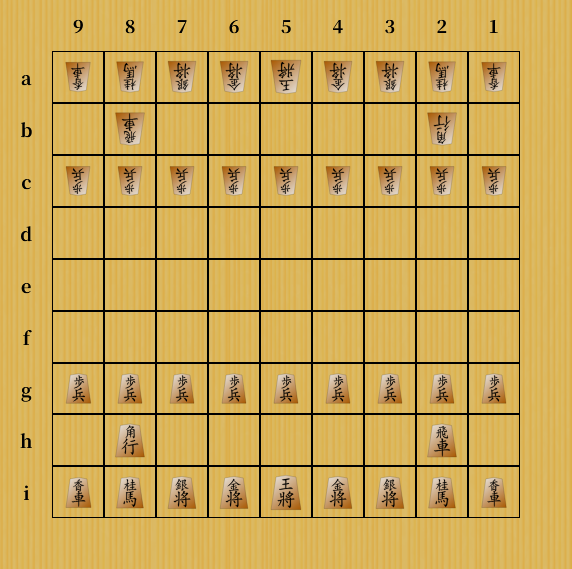
\includegraphics[width=0.9\linewidth]{images/board.png}
	\caption{Posição inicial do tabuleiro}
	\label{fig:posicao_inicial}
\end{figure}

Considere a seguinte representação SFEN correspondente à posição inicial do tabuleiro: 

\begin{center}
\small
\texttt{lnsgkgsnl/1r5b1/ppppppppp/9/9/9/PPPPPPPPP/1B5R1/LNSGKGSNL b - 1}
\end{center}
Como ilustrado na Figura~\ref{fig:posicao_inicial}, o primeiro campo descreve o tabuleiro, 
cujas linhas são separadas pelo caractere "/" e estão ordenadas de cima para baixo. As peças 
seguem a notação da Tabela~\ref{tab:shogi_pieces}. As letras minúsculas representam as peças 
do \textit{gote} e as maiúsculas representam as peças do \textit{sente}. Casas vazias são 
representadas por números que indicam a quantidade de casas consecutivas desocupadas.

O segundo campo indica que o \textit{sente} deve fazer o próximo movimento, uma vez que 
ele é o jogador que começa o jogo. O símbolo - no terceiro campo indica que nenhum deles 
possui peças capturadas disponíveis para reutilização. Por fim, o quarto campo indica que 
a próxima jogada será a primeira do jogo.
	
\section{Universal Shogi Interface}
\label{sec:USI}
No contexto do shogi computacional, os chamados motores, ou \textit{engines}, são programas 
capazes de analisar posições e buscar movimentos possíveis, utilizando algoritmos de busca 
e funções de avaliação para estimar a qualidade de diferentes jogadas. Esses motores podem 
ser integrados a interfaces gráficas, permitindo o desenvolvimento de aplicações de análise 
de partidas, como o Lishogi, que utiliza o YaneuraOu\textsuperscript{\cite{yaneuraou}}.

A comunicação entre motores e interfaces pode ser realizada por meio do protocolo 
\textit{Universal Shogi Interface} (USI), baseado no protocolo equivalente utilizado 
no xadrez \textit{Universal Chess Interface} (UCI). Ao padronizar comandos e respostas, 
o USI elimina a necessidade de implementar os mecanismos de análise dentro das próprias aplicações.

Esse protocolo define operações para inicializar o motor, configurar suas opções, fornecer 
posições do tabuleiro por meio da representação SFEN e solicitar a busca por movimentos. 
Essa comunicação ocorre através da entrada e da saída padrão do processo do motor. Durante 
uma busca, o programa pode retornar informações sobre a análise realizada, como a profundidade 
alcançada que indica quantos meios-lances (movimentos individuais de um jogador) foram explorados 
na busca, a avaliação da posição e os movimentos candidatos considerados. 
%!TeX root=../main.tex

\chapter{Trabalhos relacionados}
\label{cap:trabalhos-relacionados}

\section{Sistema de apoio ao aprendizado de shogi}
\cite{future-position} propôs um método de apoio ao aprendizado de shogi para jogadores iniciantes, 
denominado \textit{Posição Futura}. O autor observou que a apresentação explícita de movimentos recomendados por programas de shogi 
pode levar os jogadores a dependerem excessivamente das sugestões do computador, prejudicando o desenvolvimento de uma habilidade 
importante em jogos de estratégia: antecipar possíveis jogadas para tomar decisões. Para investigar como diferentes níveis de suporte 
afetam o aprendizado, ele desenvolveu um sistema que apresenta posições futuras do tabuleiro, geradas por meio de partidas entre programas 
de inteligência artificial (IA), considerando diferentes distâncias (jogadas à frente) em relação à posição atual. Dessa forma, o jogador 
recebe informações que podem auxiliar na compreensão do desenvolvimento da partida sem que uma jogada específica seja indicada diretamente.

O autor avaliou a proposta por meio de um experimento que comparou diferentes níveis de assistência durante a prática de shogi, incluindo 
uma condição sem assistência. Os resultados indicaram uma tendência de melhora nos testes após a utilização das dicas, embora o número 
reduzido de participantes não tenha permitido identificar diferenças estatisticamente significativas entre os níveis de assistência. O estudo 
sugere, portanto, que a apresentação de informações sobre o jogo pode constituir uma abordagem promissora para apoiar o aprendizado de shogi, 
embora sejam necessárias investigações adicionais. 

\section{Sistema tutor inteligente para jogos estratégicos}
No trabalho de \cite{AI-gomoku-tutor}, os autores observaram que a abordagem padrão utilizada 
por tutores humanos de jogos estratégicos, como Go, Gomoku e Shogi, foi expor jogadores iniciantes a diversas partidas e ao final analisar as 
jogadas realizadas. Dessa forma, investigaram a possibilidade de desenvolver um sistema tutor inteligente que permite que os jogadores 
aprendam a partir da revisão dos jogos, comparando essa estratégia com outros dois métodos de suporte: a apresentação de dicas ao longo da 
partida e o fornecimento de feedback imediato após cada jogada. 

Nesse contexto, foi proposto um sistema que permite ao usuário jogar Gomoku contra uma IA treinada no jogo e fornece a ele as abordagens de 
ensino mencionadas anteriormente. Para avaliar o sistema, foram conduzidos dois estudos-piloto nos quais os participantes foram distribuídos 
aleatoriamente entre as três condições de aprendizagem. No primeiro estudo, após interagirem com o sistema durante 20 minutos, os 
participantes jogaram cinco partidas de teste. Os resultados indicaram que aqueles que receberam feedback imediato apresentaram melhor 
aprendizagem do que aqueles que receberam feedback tardio. No segundo estudo, foi adotado um formato de pré-teste e pós-teste: os 
participantes responderam inicialmente a 20 questões sobre estratégias de Gomoku, utilizaram o sistema durante 35 minutos e, em seguida, 
responderam às mesmas questões em ordem diferente, com os tabuleiros rotacionados ou espelhados. Os resultados preliminares indicaram que 
os participantes de todas as condições obtiveram desempenho significativamente superior no pós-teste em relação ao pré-teste.

\section{Sistema de ensino de xadrez com grafo de conhecimento}
No trabalho de \cite{EKChess}, os autores identificaram três desafios enfrentados pelas ferramentas de ensino de xadrez: a atenção limitada dedicada ao ensino de finais de partida; a escassez de sistemas de ensino de xadrez baseados em grafos de conhecimento, estruturas que representam fatos por meio de entidades, relações e descrições semânticas; e a ausência de critérios padronizados para avaliar os resultados de aprendizagem dos participantes em processos de ensino de xadrez que utilizam inteligência artificial. 

Para abordar essas questões, os autores desenvolveram o sistema chamado \textit{EK-Chess}, que permite aos usuários jogar xadrez e receber feedback em tempo real. O sistema utiliza um grafo de conhecimento de finais de partida, construído a partir do conhecimento de especialistas,  no qual as posições são representadas por meio da notação Forsyth-Edwards (FEN) e os movimentos pela notação algébrica longa \textit{Long Algebraic Notation} (LAN). Esses elementos são organizados como nós de um grafo direcionado, que serve de base para fornecer informações sobre movimentos e explicações relacionadas a cenários específicos do jogo.

Para avaliar o sistema, os autores conduziram um experimento com 20 crianças entre 6 e 10 anos de idade, que conheciam os movimentos das peças e as regras do xadrez, mas ainda não dominavam estratégias mais avançadas, sendo consideradas no nível iniciante. Os participantes foram divididos em dois grupos, um que estudou usando o \textit{EK-Chess} e outro usando livros tradicionais. Após aprenderem a utilizar os respectivos recursos de ensino, os participantes de ambos os grupos responderam a um teste antes e outro depois do período de estudo. As questões apresentavam diferentes níveis de dificuldade, definidos de acordo com o conhecimento necessário para chegar à resposta correta.

Os resultados indicaram que os participantes que utilizaram o EK-Chess obtiveram melhor desempenho no pós-teste, especialmente nas questões de dificuldade intermediária. No grupo que utilizou livros, também foi observado um desempenho melhor nessas questões, mas sem uma melhora estatisticamente significativa no resultado geral, conforme relatado pelos autores. Os resultados, portanto, sugerem que o EK-Chess pode contribuir para o aprendizado de estratégias de xadrez.

Os autores argumentam que uma das principais diferenças entre os métodos de ensino está na presença de um mecanismo de registro do progresso no sistema, que permite aos usuários identificar as etapas já concluídas e aquelas que ainda precisam ser realizadas. Segundo os autores, esse mecanismo pode reduzir a carga cognitiva associada ao acompanhamento do próprio aprendizado, contribuindo para a eficácia do processo de ensino. Além disso, discutem a possibilidade de utilizar os dados registrados durante o aprendizado em conjunto com sistemas de recomendação, permitindo modelar as preferências e o domínio do conteúdo por cada usuário para oferecer recomendações de estudo personalizadas e, potencialmente, melhorar os resultados de aprendizagem.

Por fim, os autores exploram a possibilidade de utilizar o grafo de conhecimento desenvolvido para fornecer informações a LLMs (\textit{Large Language Models}), visando aprimorar seu desempenho em tarefas relacionadas ao xadrez.

\section{Korbit}
\cite{korbit-article} investigaram o uso de técnicas automatizadas para selecionar feedback em sistemas tutores inteligentes, considerando as características das orientações disponíveis e os dados relacionados ao desempenho e às interações anteriores dos estudantes. Os autores buscaram avaliar se a personalização desse processo poderia contribuir para melhorar os resultados de aprendizagem.

Para avaliar essa abordagem, os autores realizaram um experimento com 183 estudantes de \textit{Machine Learning} (ML) que precisaram utilizar uma plataforma de ensino online chamada \textit{Korbit}\textsuperscript{\cite{korbit-site}} (um sistema tutor inteligente baseado em diálogo que emprega técnicas ML, processamento de linguagem natural (PLN) e aprendizado por reforço para oferecer uma experiência de aprendizagem interativa e personalizada) durante um mês.

Os autores investigaram três tipos de feedback automático: dicas e explicações geradas por meio de técnicas de processamento de linguagem natural (PLN); explicações extraídas de artigos da Wikipédia sobre aprendizado de máquina; e dicas para problemas matemáticos, incluindo equações incompletas e orientações para corrigir equações incorretas. Para selecionar as dicas personalizadas, foram avaliados três modelos: \textit{baseline}, que considera características linguísticas das dicas, como seu tamanho e a sobreposição de palavras-chave com a pergunta; \textit{shallow personalization}, que utiliza características relacionadas ao desempenho do estudante, como a quantidade de questões tentadas e a proporção de respostas corretas e incorretas; e \textit{deep personalization}, que também considera características linguísticas de até quatro interações anteriores entre o estudante e o sistema.

O ganho de aprendizagem foi avaliado pela proporção de questões inicialmente respondidas incorretamente que passaram a ser respondidas corretamente após o recebimento de uma dica ou explicação. Os autores analisaram essa métrica considerando todos os estudantes e, separadamente, aqueles que receberam feedback antes da segunda tentativa. Os resultados indicaram que o modelo \textit{deep personalization} apresentou o maior ganho de aprendizagem, enquanto o \textit{baseline} apresentou o menor, na análise que considerou todos os estudantes. Na análise restrita aos estudantes que receberam feedback antes da segunda tentativa, a diferença entre o modelo \textit{deep personalization} e o \textit{baseline} foi estatisticamente significativa. Esses resultados sugerem que considerar informações sobre o desempenho e as interações anteriores dos estudantes pode contribuir para a eficácia do feedback em sistemas tutores inteligentes.  

\section{Comparação com o Shogi-sensei}
Diferentemente do sistema de Ito e do tutor de gomoku, que utilizam partidas ou trechos delas para ensinar conceitos dos jogos abordados, o Shogi-sensei fornece diferentes
tipos de exercícios, cada um focado em um conceito específico e só avançando para conceitos mais avançados quando o usuário apresentar um domínio adequado do conteúdo
estudado naquele momento.

Enquanto o EK-Chess utiliza um grafo de conhecimento como base para fornecer informações e explicações relacionadas ao jogo, o Korbit utiliza características linguísticas das 
orientações, informações sobre o desempenho dos estudantes e dados de interações anteriores. A estratégia abordada pelo Shogi-sensei, por outro lado, utiliza um LLM, que 
recebe um prompt (Figura~\ref{fig:prompt}) contendo instruções para gerar as explicações.  

Por fim, os trabalhos apresentados avaliaram suas propostas por meio de diferentes abordagens, incluindo a comparação entre condições de aprendizagem, a aplicação de 
testes antes e depois das atividades e a análise do desempenho dos estudantes após o recebimento de feedback. Neste trabalho, a avaliação considera métricas como a taxa de 
acerto e a variação da distribuição de probabilidades de seleção atribuídas a cada módulo, permitindo analisar tanto o desempenho dos usuários, segundo os critérios 
estabelecidos pelo sistema, quanto o funcionamento do mecanismo de recomendação de exercícios.
%!TeX root=../main.tex

\chapter{Desenvolvimento}
\label{cap:desenvolvimento}

    O sistema do Shogi-sensei pode ser dividido em quatro blocos principais: o banco de dados, a \textit{engine} do YaneuraOu, o servidor e por fim a interface. A relação entre esses componentes é apresentada na Figura~\ref{fig:system_overview}. Cada bloco foi desenvolvido em um \textit{docker container} diferente, com o intuito de permitir que o projeto possa ser executado em qualquer máquina.

    \begin{figure}[H]
        \centering
        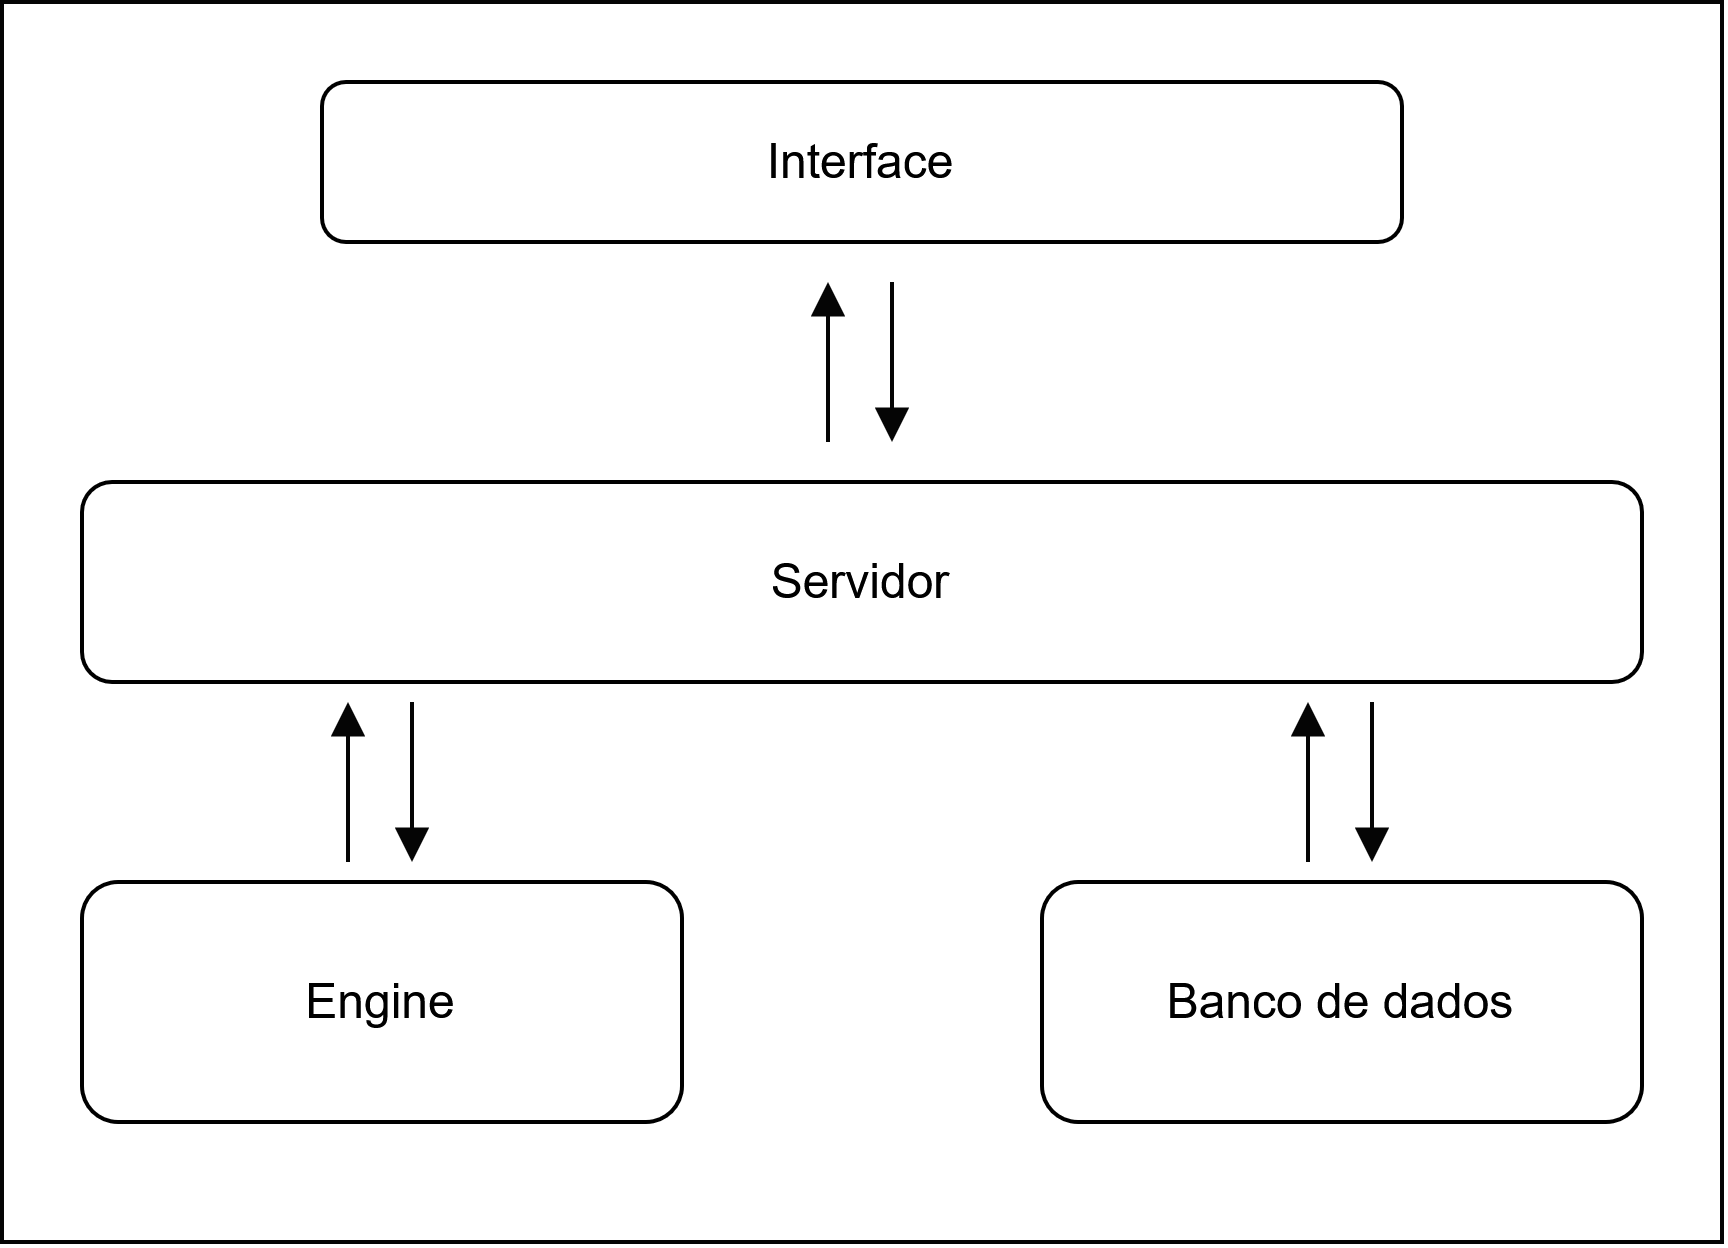
\includegraphics[width=0.9\linewidth]{images/system_overview.png}
        \caption{Visão geral do sistema}
        \label{fig:system_overview}
    \end{figure}

    \begin{figure}[H]
        \centering
        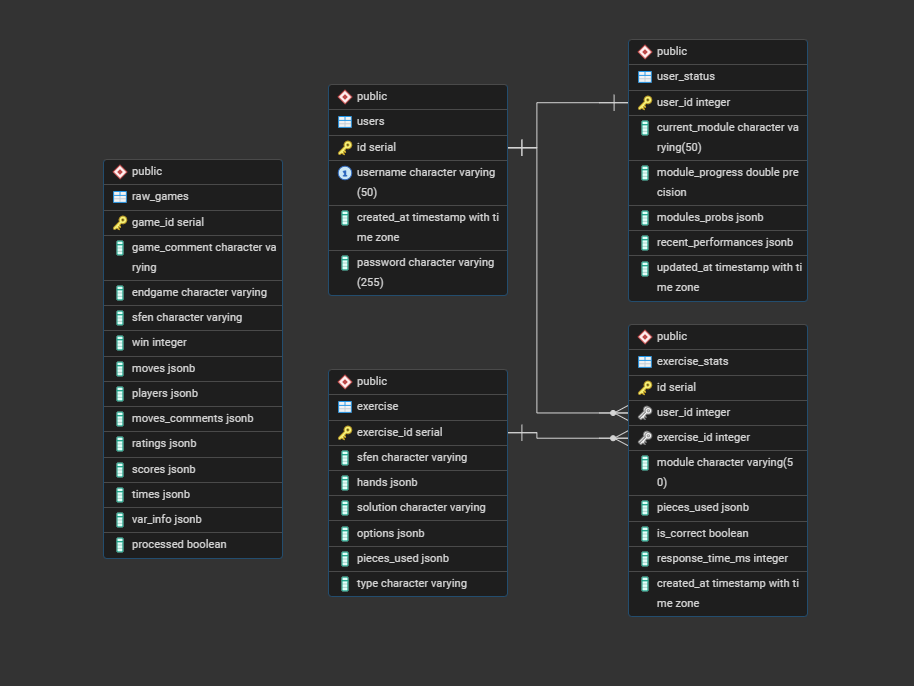
\includegraphics[width=0.9\linewidth]{images/tables.png}
        \caption{Tabelas do banco de dados}
        \label{fig:db_tables}
    \end{figure}
    
     \section{Banco de dados}
     \label{sec:database}
    O sistema utiliza o \textit{PostgreSQL} para armazenar informações dos usuários e dos exercícios. A escolha desse sistema foi motivada pela experiência prévia do autor com a ferramenta e pela facilidade de integração com Python por meio de bibliotecas como \textit{SQLAlchemy}, utilizada para definir modelos e realizar operações sobre os dados; \textit{psycopg}, responsável pela comunicação com o banco de dados; e \textit{Alembic}, empregado para gerenciar alterações no esquema do banco por meio de migrações. As tabelas são apresentadas na Figura~\ref{fig:db_tables} e são descritas abaixo:

    \begin{itemize}
        \item \textbf{raw\_games}: armazena os dados brutos de partidas extraídas da plataforma WDoor\textsuperscript{\cite{wdoor}}, que disponibiliza partidas no formato CSA, apresentado na seção~\ref{sec:server}.
        \item \textbf{users}: armazena os dados de cadastro dos usuários do sistema, incluindo o hash da senha, em vez da senha original.
        \item \textbf{user\_status}: contém informações referentes ao progresso do usuário. 
        \begin{itemize}
            \item \textbf{current\_module}: identifica o módulo em que o usuário se encontra.
            \item \textbf{module\_progress}: registra o progresso do usuário no módulo atual.
            \item \textbf{modules\_probs}: armazena a distribuição de probabilidades utilizada para orientar a recomendação dos módulos de exercícios.
            \item \textbf{recent\_performances}:  mantém um histórico do desempenho do usuário nos módulos.
        \end{itemize}
        \item \textbf{exercise}: contém os dados dos exercícios gerados.
        \begin{itemize}
            \item \textbf{sfen}: representação SFEN do estado do tabuleiro.
            \item \textbf{hands}: peças que cada jogador tem em mãos.
            \item \textbf{solution}: solução do exercício.
            \item \textbf{options}: alternativas do exercício, que incluem a solução.
            \item \textbf{pieces\_used}: peças utilizadas na solução do exercício.
            \item \textbf{type}: módulo ao qual o exercício pertence.
        \end{itemize}
        \item \textbf{exercise\_stats}: armazena as estatísticas das respostas enviadas pelos usuários para os exercícios.
        \begin{itemize}
            \item \textbf{user\_id}: identificação única do usuário.
            \item \textbf{exercise\_id}: identificação única do exercício.
            \item \textbf{module}: módulo ao qual o exercício pertence.
            \item \textbf{pieces\_used}: mesmo campo presente na tabela \textbf{exercise}.
            \item \textbf{is\_correct}:  indica se a resposta foi correta (True) ou incorreta (False).
            \item \textbf{response\_time}: tempo, em milissegundos, gasto pelo usuário para responder ao exercício.
        \end{itemize}
    \end{itemize}

    \section{\textit{Engine}}
    Assim como mencionado no início desta seção, o sistema utiliza a \textit{engine} YaneuraOu, baseada em um modelo NNUE (\textit{Efficiently Updatable Neural Network}). Escolheu-se essa \textit{engine} por não depender de uma placa de vídeo poderosa, o que viabilizou usá-la num ambiente local. Como a comunicação com o YaneuraOu ocorre através do envio de comandos USI pela entrada do próprio processo e lê-se a saída devolvida, optou-se por separá-lo do servidor. Assim, utilizou-se a biblioteca \textit{FastAPI} para criar um serviço que realiza a comunicação entre os dois processos, com o benefício do servidor não ser prejudicado quando a \textit{engine} apresentar algum erro.

    \begin{figure}[H]
        \centering
        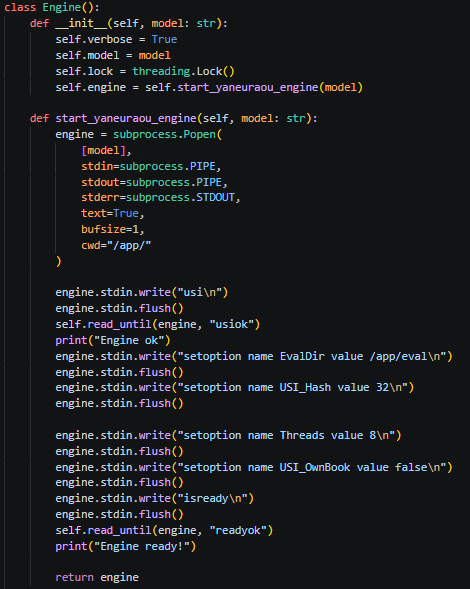
\includegraphics[width=0.9\linewidth]{images/engine_init.png}
        \caption{Inicialização da \textit{engine}}
        \label{fig:engine_init}
    \end{figure}

    Para inicializar o YaneuraOu, envia-se o comando \textit{usi}. Após ele enviar a mensagem \textit{usiok}, envia-se o comando 
    \textit{setoption name EvalDir value <path>}, onde \textit{path} se refere ao caminho para o diretório que contém os pesos da rede neural utilizada na avaliação das posições. Em seguida, são realizadas algumas configurações de desempenho. Por fim, envia-se o comando \textit{isready} e, após a \textit{engine} enviar \textit{readyok}, a inicialização está finalizada.
    
    Embora inicialmente estivesse previsto o uso do YaneuraOu na geração de exercícios de todos os módulos, durante o desenvolvimento verificou-se que ele seria necessário apenas no módulo de xeque-mate em um lance, no qual é empregado para auxiliar na geração de alternativas de resposta. O processo de geração dessas alternativas é apresentado na seção~\ref{sec:server}.
    
    \section{Servidor}
    \label{sec:server}
    Para o desenvolvimento do servidor, utilizou-se a biblioteca \textit{FastAPI}, responsável pela criação e pelo gerenciamento dos endpoints da API consumida pela interface do sistema. Esse componente ficou responsável pelas seguintes funcionalidades:
    
    \begin{itemize}
    \item Gerar os exercícios automaticamente;
    \item Organizar os exercícios em listas;
    \item Corrigir os exercícios e gerar a explicação;
    \item Realizar o cadastro e a autenticação dos usuários;
    \item Atualizar e consultar as estatísticas de desempenho dos usuários;
    \item Gerenciar a comunicação com o banco de dados.
    \end{itemize}

    \subsection{Arquitetura}
    O servidor utiliza uma arquitetura em camadas, com o objetivo de separar as responsabilidades dos componentes do sistema, facilitando sua manutenção e isolando a implementação de cada funcionalidade. Dessa forma, o código foi organizado em três camadas:
    \begin{itemize}
        \item Repositórios: responsáveis por realizar as operações de persistência e consulta de dados no banco de dados.
        \item Serviços:  responsáveis por implementar e gerenciar a lógica de funcionamento do sistema.
        \item Roteadores: responsáveis por definir os endpoints da API, recebendo as requisições dos clientes e encaminhando-as aos serviços correspondentes.
    \end{itemize}

    Durante o processamento de uma requisição, o roteador aciona o serviço responsável pela funcionalidade solicitada, que, quando necessário, utiliza os repositórios para acessar o banco de dados. O fluxo é representado na Figura~\ref{fig:server_architecture}.

    \begin{figure}[H]
        \centering
        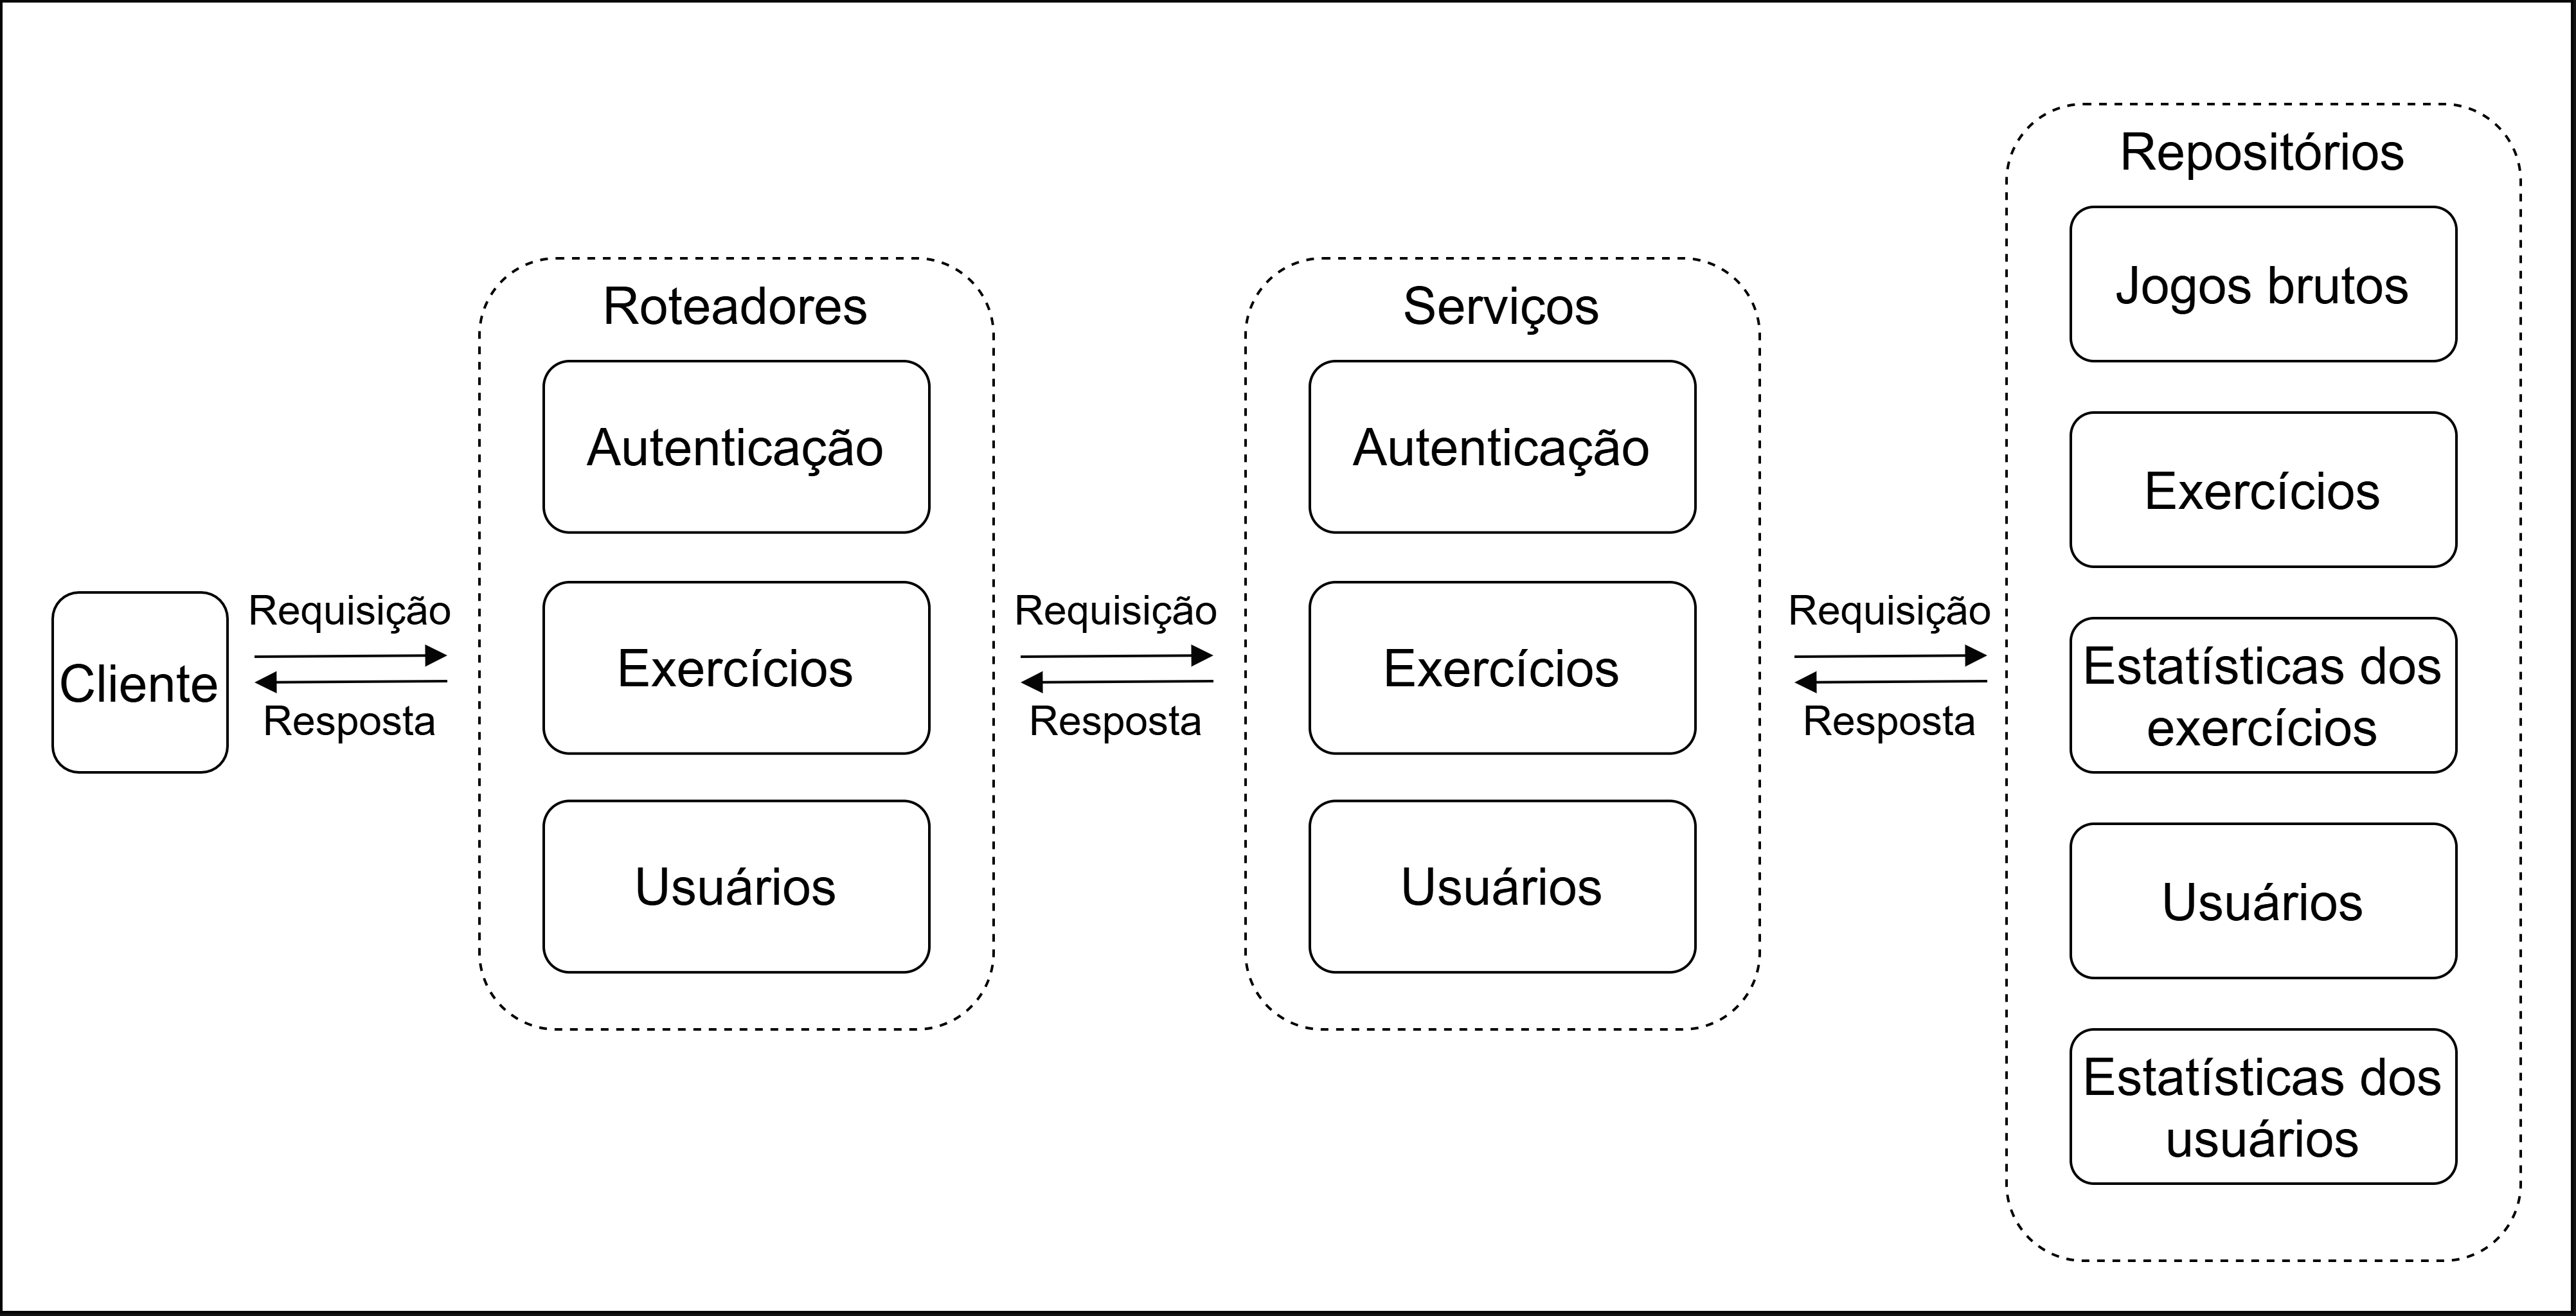
\includegraphics[width=1.0\linewidth]{images/server_architecture.png}
        \caption{Arquitetura do servidor}
        \label{fig:server_architecture}
    \end{figure}
    
    Além dessas camadas, foram utilizados esquemas do Pydantic para estruturar e validar os dados recebidos e retornados pelos endpoints, garantindo um formato padronizado para a comunicação entre o cliente e o servidor.


    \subsection{Geração automática de exercícios}
    Para padronizar a apresentação dos exercícios e simplificar a sua implementação na interface, todas as questões consideram que é a vez do jogador \textit{sente} de jogar.
    Cada questão apresenta quatro alternativas, das quais apenas uma é a correta, e pertence a um dos seguintes módulos:
    \begin{itemize}
        \item \textbf{Reconhecimento}: pede para que o usuário identifique uma determinada peça no tabuleiro.
        \item \textbf{Movimento 1}: apresenta apenas uma peça sem o símbolo escrito no tabuleiro com seus movimentos destacados e pede para que o usuário identifique qual seria tal peça.
        \item \textbf{Movimento 2}: semelhante ao Movimento 1, mas existem outras peças no tabuleiro que impedem alguns movimentos.
        \item \textbf{Promoção}: pede para que o usuário identifique qual movimento pode levar a uma promoção. 
        \item \textbf{Drop}: pede para que o usuário identifique qual movimento constitui um \textit{drop} legal.
        \item \textbf{Xeque-mate}: pede para que o usuário identifique qual movimento leva ao xeque-mate.
    \end{itemize}

    Assim como mencionado na seção~\ref{sec:database}, os exercícios são gerados a partir de uma plataforma que contém partidas entre jogadores reais, com o intuito de garantir que as posições apresentadas no tabuleiro são legais e expor os usuários do sistema a cenários encontrados em partidas reais. Esses jogos são disponibilizados no formato CSA, arquivos que contêm informações como nome dos jogadores, registro dos movimentos, estado do tabuleiro ao final da partida no formato SFEN e qual foi o vencedor.
    Para processar os dados dos jogos, foi utilizada uma biblioteca chamada \textit{cshogi}\textsuperscript{\cite{cshogi}}, que permite manipular um tabuleiro de shogi, extrair informações, como a posição das peças e as mãos de cada jogador a partir da representação SFEN, simular movimentos e verificar a legalidade das jogadas. Dessa forma, para cada jogo, a geração segue os passos abaixo:

    \begin{enumerate}
        \item Simulação dos movimentos registrados;
        \item Para cada movimento, são definidas a solução e as opções de acordo com os critérios de cada módulo.
        \item Registro desse exercício em uma lista para o posterior registro no banco de dados.
    \end{enumerate}

    Mais detalhes do passo 2 estão descritos abaixo:

    \begin{itemize}
        \item \textbf{Reconhecimento}:
        A solução consiste em selecionar aleatoriamente uma peça no tabuleiro. As alternativas são compostas pela solução e outras três peças diferentes. Por exemplo, se um peão é escolhido como solução, as outras alternativas podem ser lança, cavalo e rei.
        \item \textbf{Movimento 1}: Nesse módulo, não é necessário utilizar os jogos extraídos da plataforma. Para cada uma das 14 peças possíveis, é definido um tabuleiro que contém apenas essa peça em sua região central, representado pelo SFEN 9/9/9/9/<peça>/ 9/9/9/9. Em seguida, as alternativas são selecionadas entre as peças restantes que apresentam padrões de movimento diferentes do padrão da solução, evitando a possibilidade de mais de uma resposta correta. Por exemplo, caso a solução seja um general de ouro, as alternativas não poderão incluir peças promovidas, com exceção da torre e do bispo promovidos, pois as demais possuem o mesmo padrão de movimento do general de ouro.
        \item \textbf{Movimento 2}: Diferentemente do módulo Movimento 1, uma peça presente no tabuleiro de uma partida real é selecionada aleatoriamente para ser a solução. As alternativas são determinadas seguindo o mesmo critério do módulo anterior. Entretanto, a presença de outras peças no tabuleiro pode restringir os movimentos disponíveis, adicionando uma camada de dificuldade, pois nem todos os movimentos possíveis de uma peça estarão necessariamente disponíveis na posição apresentada.  
        \item \textbf{Promoção}: Inicialmente, é selecionado aleatoriamente um movimento que permite a promoção de uma peça. Durante a seleção das alternativas, são descartados os movimentos que também resultariam na promoção de uma peça. Além disso, para cada movimento de promoção descartado, também é eliminado o movimento correspondente sem promoção, mesmo que nenhum dos dois corresponda à solução. Isso evita que duas alternativas representem a mesma jogada, diferenciando-se apenas pela decisão de promover ou não a peça. Por exemplo, se a solução for 8d->8c+ e uma das alternativas possíveis for 7d->7c+, esta última será descartada, assim como 7d->7c.
        \item \textbf{Drop}: O processo é semelhante ao módulo Promoção. Um movimento de drop é escolhido aleatoriamente e definido como a solução do exercício. Em seguida, os demais movimentos de drop legais são descartados. Por fim, as alternativas são constituídas por movimentos de drop ilegais, como o posicionamento de um peão em uma coluna que já contém outro peão aliado.
        \item \textbf{Xeque-mate}: Verifica-se se determinado movimento resulta em xeque-mate. Caso isso ocorra, o movimento identificado e o estado do tabuleiro são enviados para a \textit{engine}, responsável pela geração das alternativas. Seu uso nesse processo permite selecionar movimentos candidatos com base na posição, tornando as alternativas mais plausíveis e, consequentemente, aumentando a dificuldade do exercício. Isso evita que movimentos claramente distantes da região onde se encontra o rei adversário evidenciem facilmente a resposta correta. Por exemplo, suponha que a solução seja mover um general de ouro da casa 4d para a casa 5c. Caso as alternativas incluam movimentos de peões para casas distantes do rei adversário, como as linhas g ou h, torna-se mais fácil identificar a solução. No entanto, é possível que dentre os movimentos escolhidos pelo YaneuraOu, exista mais de um xeque-mate. Dessa forma, esses movimentos são também excluídos.
        
    \end{itemize}
%!TeX root=../main.tex

\chapter{Metodologia}
\label{cap:metodologia}

Para avaliar o sistema proposto neste trabalho, foi realizado um experimento com 15 participantes sem conhecimento prévio de shogi, durante um período de três semanas. Ao longo desse período, os participantes foram instruídos a resolver pelo menos uma lista de exercícios por dia, utilizando o sistema.

Durante o experimento, foram coletadas métricas relacionadas ao desempenho dos participantes, incluindo o tempo de resposta, a taxa média de acertos por módulo e a quantidade de listas necessárias para avançar para o módulo seguinte. Essas métricas permitiram analisar o desempenho dos usuários e o funcionamento da progressão de dificuldade implementada no sistema.

Ao final do experimento, foi disponibilizado um questionário para coletar as opiniões dos participantes sobre diferentes aspectos do sistema, como usabilidade, organização dos módulos, dificuldade dos exercícios e contribuição para o aprendizado. O questionário foi composto pelas seguintes perguntas:

\begin{itemize}
    \item De 1 a 10, você considera a interface intuitiva e fácil de utilizar?
    \item Qual foi o módulo que você teve mais dificuldade?
    \item Qual o motivo?
    \item A progressão dos módulos faz sentido? Por que?
    \item Você considera que a quantidade de exercícios por lista é a ideal? Por que?
    \item Você considera que aprendeu os fundamentos básicos do shogi após utilizar o sistema? Por que?
    \item De 1 a 10, você considera que as explicações apresentadas pelo sistema são claras e fáceis de compreender?
    \item De 1 a 10, o quanto você considera que as explicações ao final das listas contribuiu para o seu aprendizado?
    \item Você tem alguma sugestão de pontos a melhorar no sistema?
\end{itemize}
%!TeX root=../main.tex

\chapter{Resultados}
\label{cap:resultados}

Este capítulo apresenta os resultados obtidos durante o experimento, acompanhados de uma discussão sobre os dados coletados. Inicialmente, 
são analisadas as métricas de desempenho dos participantes, com o objetivo de avaliar o funcionamento do sistema de recomendação de 
exercícios e investigar  a contribuição da abordagem de ensino e das explicações fornecidas pela IA para o aprendizado. Em seguida, 
são apresentadas e discutidas as respostas ao questionário aplicado, buscando compreender a experiência dos participantes e identificar 
possíveis pontos de melhoria no sistema.

\section{Desempenho dos usuários}
\label{sec:users_performances}
Na Tabela~\ref{tab:piece_accuracy}, são apresentadas as taxas de acerto por peça em cada módulo, acompanhadas da quantidade de exercícios em que cada uma aparece.

Destaca-se a predominância do Peão entre os exercícios, o que pode ser explicado, principalmente, por sua maior quantidade no tabuleiro, aumentando a 
probabilidade de ser selecionado pelo gerador de questões. Em contrapartida, as peças promovidas aparecem com menor frequência, devido à sua menor disponibilidade 
nas posições utilizadas para a geração dos exercícios.

\begin{table}[H]
\centering
\caption{Taxa de acerto por peça}
\label{tab:piece_accuracy}
\small
\resizebox{\textwidth}{!}{%
\begin{tabular}{>{\centering\arraybackslash}m{1.2cm} >{\centering\arraybackslash}m{1.7cm} >{\centering\arraybackslash}m{1.7cm} >{\centering\arraybackslash}m{1.7cm} >{\centering\arraybackslash}m{1.7cm} >{\centering\arraybackslash}m{1.7cm} >{\centering\arraybackslash}m{1.7cm} >{\centering\arraybackslash}m{1.7cm}}
\toprule
Peça & \makecell{Reconhe-\\cimento} & Movimento 1 & Movimento 2 & Promoção & Drop & Xeque-mate & Total \\
\midrule
+B & 60.0\% (10) & 94.6\% (74) & 100.0\% (2) & — & — & 62.5\% (8) & 88.3\% (94) \\ \midrule
+L & 75.0\% (4) & 85.9\% (78) & — & — & — & 50.0\% (4) & 83.7\% (86) \\ \midrule
+N & 71.4\% (7) & 82.4\% (91) & — & — & — & — & 81.6\% (98) \\ \midrule
+P & 95.8\% (24) & 83.6\% (61) & 0.0\% (2) & — & — & 100.0\% (2) & 85.4\% (89) \\ \midrule
+R & 81.0\% (21) & 97.6\% (82) & 100.0\% (2) & — & — & 76.9\% (26) & 90.8\% (131) \\ \midrule
+S & 100.0\% (2) & 84.5\% (84) & — & — & — & — & 84.9\% (86) \\ \midrule
B & 88.4\% (43) & 96.8\% (63) & 96.7\% (30) & 91.1\% (235) & 95.7\% (188) & 54.5\% (11) & 92.6\% (570) \\ \midrule
G & 87.7\% (195) & 94.0\% (67) & 91.2\% (113) & — & 94.0\% (84) & 77.1\% (83) & 88.6\% (542) \\ \midrule
K & 87.3\% (110) & 97.3\% (74) & 98.6\% (70) & — & — & — & 93.3\% (254) \\ \midrule
L & 89.2\% (176) & 95.8\% (72) & 90.7\% (54) & 92.7\% (41) & 85.7\% (56) & 66.7\% (6) & 90.1\% (405) \\ \midrule
N & 95.7\% (185) & 93.8\% (65) & 100.0\% (36) & 97.3\% (113) & 80.2\% (81) & 71.4\% (7) & 93.2\% (487) \\ \midrule
P & 95.4\% (723) & 96.1\% (76) & 99.7\% (311) & 94.5\% (164) & 82.2\% (259) & 50.0\% (2) & 93.9\% (1535) \\ \midrule
R & 91.0\% (89) & 94.0\% (83) & 97.6\% (42) & 94.0\% (184) & 100.0\% (30) & 76.9\% (13) & 93.7\% (441) \\ \midrule
S & 85.5\% (186) & 88.9\% (72) & 88.0\% (100) & 88.0\% (75) & 94.4\% (72) & 87.5\% (8) & 88.1\% (513) \\
\bottomrule
\end{tabular}
}
\end{table}

Os gráficos do Apêndice~\ref{ap:modules_performances} apresentam a taxa de acerto de cada participante por módulo. Entretanto, como uma mesma lista pode conter 
exercícios de diferentes módulos, a quantidade de questões de cada tipo pode variar consideravelmente. Dessa forma, essa métrica deve ser interpretada com cautela, 
pois, quanto menor a quantidade de exercícios de determinado módulo, maior pode ser o impacto de uma única resposta incorreta sobre a taxa de acerto.

Os gráficos do Apêndice~\ref{ap:avg_response_time}, por sua vez, apresentam o tempo médio de resposta de cada participante por lista e módulo. De maneira geral, observa-se uma tendência de 
redução desse tempo ao longo das listas, o que pode indicar maior familiaridade dos participantes com os exercícios e os conceitos abordados. Entretanto, essa redução, 
isoladamente, não permite concluir que houve retenção do conteúdo.

Por fim, os gráficos do Apêndice~\ref{ap:modules_probs}, permitem observar a evolução da distribuição de probabilidades atribuídas a cada módulo ao longo das listas 
respondidas. Como o mecanismo adaptativo reduz a probabilidade de seleção dos módulos nos quais o participante apresenta taxa de acerto igual ou superior a 70\%, 
enquanto aumenta a dos módulos com desempenho inferior a esse limite, a redução das probabilidades pode indicar um desempenho satisfatório nos respectivos conteúdos.

Um comportamento que merece destaque são as quedas acentuadas e repentinas observadas em alguns módulos. Essas alterações ocorrem justamente quando um novo módulo é 
desbloqueado, recebendo inicialmente 80\% de probabilidade de seleção. Como consequência, a normalização da distribuição provoca uma redução proporcional nas probabilidades 
dos módulos já disponíveis. Dessa forma, essas quedas refletem principalmente a introdução de novos conteúdos na distribuição adaptativa.


\section{Questionário}
\subsection{Interface}
    \begin{figure}[H]
        \centering
        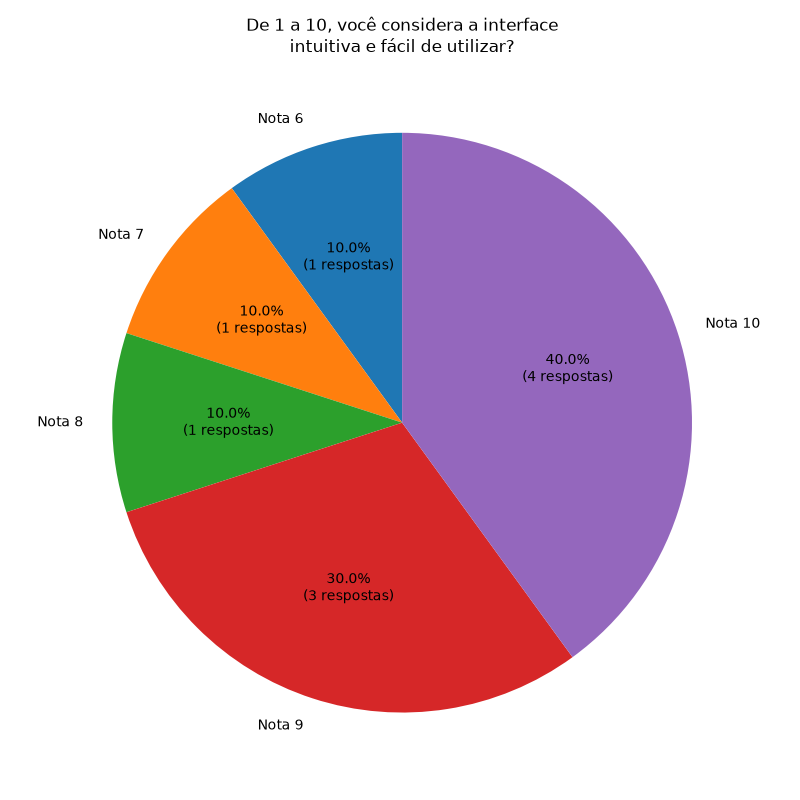
\includegraphics[width=0.9\linewidth]{images/interface_eval.png}
        \caption{Avaliação da usabilidade da interface}
        \label{fig:interface_eval}
    \end{figure}
    A Figura~\ref{fig:interface_eval} mostra que a interface foi em geral bem avaliada pelos participantes. As principais críticas envolveram:
    \begin{itemize}
        \item O contraste entre a fonte e a cor dos botões; 
        \item A notação presente nas alternativas, que dificultava a resolução da questão;
        \item O resultado da questão, que poderia ser apresentado logo após a submissão da resposta para saber se a resposta está correta 
    \end{itemize}


\subsection{Módulos mais difíceis}
    \begin{table}[H]
        \centering
        \caption{Módulos considerados mais difíceis pelos participantes}
        \label{tab:hardest_modules}
        \small
        \begin{tabular}{>{\centering\arraybackslash}m{3cm} >{\centering\arraybackslash}m{3cm} >{\centering\arraybackslash}m{8cm}}
\toprule
Módulo & Quantidade de participantes & Motivos \\
\midrule
Reconhecimento & 2 & \begin{itemize}\item Dificuldade em decorar as peças\item Explicações repetitivas e pouco úteis\end{itemize} \\\midrule
Movimento 1 & 0 & — \\\midrule
Movimento 2 & 1 & \begin{itemize}\item Dificuldade em diferenciar peças com movimentos semelhantes, principalmente as promovidas\end{itemize} \\\midrule
Promoção & 2 & \begin{itemize}\item Dificuldade em verificar todas alternativas apenas com a notação utilizada\item Explicações da IA insuficientes para compreender o conceito trabalhado\end{itemize} \\\midrule
Drop & 1 & \begin{itemize}\item Explicações da IA insuficientes para compreender o conceito trabalhado\end{itemize} \\\midrule
Xeque-mate & 4 & \begin{itemize}\item Maior dificuldade em analisar as alternativas e aplicar o raciocínio lógico\end{itemize} \\
\bottomrule
\end{tabular}


    \end{table}
 
\subsection{Progressão dos módulos}
A progressão dos módulos foi avaliada positivamente por 90\% dos participantes. Entre as justificativas apresentadas, 
destacaram-se a evolução gradual do nível de dificuldade e a construção de uma base de conhecimento, começando pelo 
reconhecimento das peças e seus movimentos antes de abordar mecânicas mais complexas, como promoção, drop e xeque-mate. 
Também foi mencionado que essa organização facilita a assimilação dos conceitos.

O participante restante não expressou uma avaliação direta sobre a progressão, mas apontou a ausência de um módulo 
introdutório que apresentasse as regras gerais do shogi, incluindo a disposição inicial das peças e o objetivo do jogo. 

\subsection{Quantidade de exercícios}
A quantidade de exercícios por lista foi considerada ideal por 80\% dos participantes, destacando que com isso foi possível
fixar melhor o conteúdo aprendido e revisar conceitos anteriores. Por outro lado, a principal crítica feita ao tamanho das listas
foi a repetitividade das questões, que, associada à ausência de explicações mais lúdicas, tornou a experiência de aprendizado menos 
dinâmica e as listas excessivamente longas.

\subsection{Compreensão dos fundamentos}
Todos os participantes consideraram que conseguiram aprender, ao menos parcialmente, os fundamentos básicos do shogi propostos pelo sistema. 
Entre as justificativas, destacaram-se a organização do conteúdo em módulos e a repetição dos exercícios, que contribuíram para a memorização 
das peças e de seus movimentos. Também foi mencionada a facilidade proporcionada pelas semelhanças com o xadrez e, em um caso, pelo conhecimento
prévio dos kanjis.

Por outro lado, alguns participantes relataram dificuldades na compreensão de conceitos específicos, principalmente as regras de promoção e drop. 
Além disso, houve críticas à qualidade das explicações fornecidas pela IA, consideradas insuficientes para esclarecer determinados erros, o que levou 
alguns participantes a recorrerem a materiais externos para complementar o aprendizado.

\subsection{Clareza e contribuição das explicações}
    \begin{figure}[H]
        \centering
        \begin{subfigure}{0.48\textwidth}
            \centering
            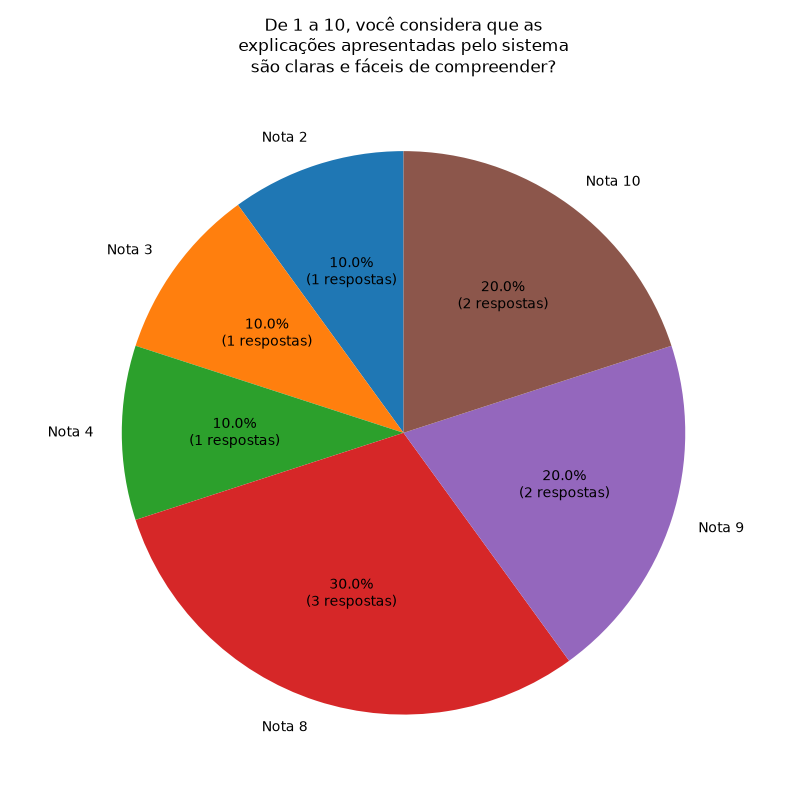
\includegraphics[width=\linewidth]{images/explanation_clarity_eval.png}
            \caption{Clareza das explicações}
            \label{fig:explanation_clarity_eval}
        \end{subfigure}
        \hfill
        \begin{subfigure}{0.48\textwidth}
            \centering
            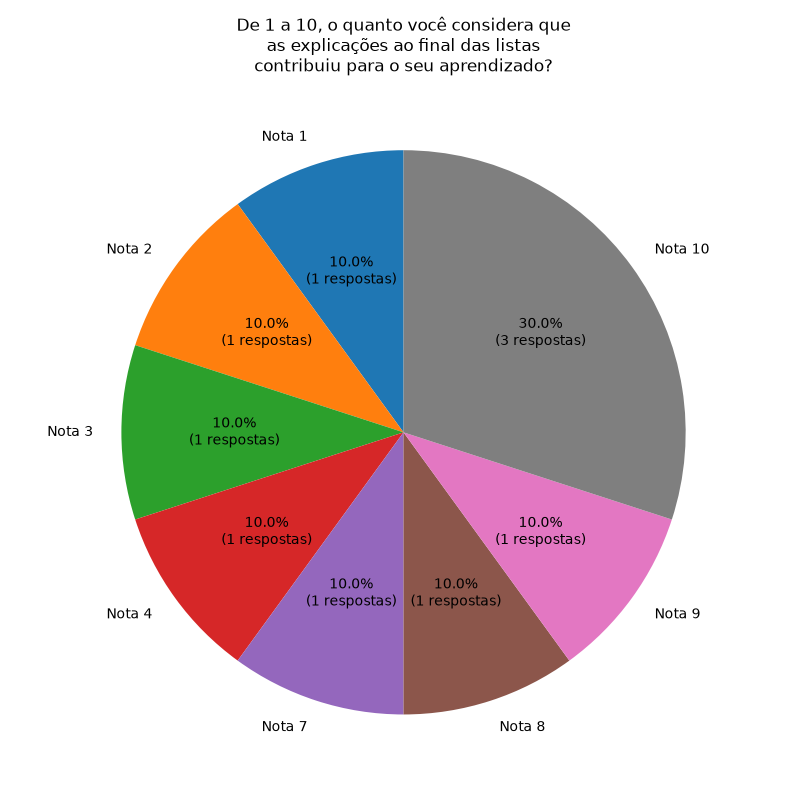
\includegraphics[width=\linewidth]{images/explanation_contribution_eval.png}
            \caption{Contribuição para o aprendizado}
            \label{fig:explanation_contribution_eval}
        \end{subfigure}
        \caption{Avaliação das explicações apresentadas pelo sistema}
        \label{fig:explanation_eval}
    \end{figure}

Conforme apresentado na Figura~\ref{fig:explanation_clarity_eval}, a clareza das explicações foi majoritariamente avaliada de forma positiva. 
Entretanto, essa percepção não se refletiu necessariamente na contribuição para o aprendizado, conforme observado na Figura~\ref{fig:explanation_contribution_eval}, 
cujas avaliações apresentaram maior variação.

As justificativas indicam que, embora as explicações tenham auxiliado alguns participantes a compreender os erros cometidos e consolidar os conceitos trabalhados, 
em determinadas situações foram consideradas vagas, confusas ou insuficientes para esclarecer o raciocínio por trás da resposta correta. Essa limitação também foi 
apontada entre as dificuldades relatadas na Tabela~\ref{tab:hardest_modules}.

Além disso, um participante destacou que a ausência de explicações para respostas corretas também pode prejudicar o aprendizado. Isso ocorre porque, ao acertar 
uma questão por eliminação ou tentativa, o usuário pode deixar de compreender o conceito envolvido, uma vez que não recebe uma explicação que justifique a alternativa selecionada.



\subsection{Sugestões de melhorias}

Entre os principais pontos de melhoria identificados pelos participantes, destacaram-se a inclusão de um módulo introdutório para apresentar os conceitos e as regras gerais 
do shogi antes do início das atividades e a distribuição dos exercícios entre as diferentes peças, especialmente as promovidas, já discutida na Seção~\ref{sec:users_performances}. 
Também foram sugeridas melhorias na visualização das peças e de seus movimentos no tabuleiro, de modo a facilitar a identificação das alternativas e reduzir a dependência da 
notação utilizada.

Além disso, alguns participantes apontaram a necessidade de diversificar os exercícios, reduzindo sua repetitividade e incluindo questões mais desafiadoras, assim como introduzir 
elementos lúdicos que incentivem a continuidade do aprendizado. Outras sugestões envolveram a disponibilização de feedback imediato após o envio das respostas e o aprimoramento das 
explicações geradas pela IA, para que apresentem justificativas mais contextualizadas e auxiliem na compreensão dos erros cometidos. Por fim, foi sugerida a inclusão de um módulo de 
prática interativa, permitindo que os usuários joguem partidas e recebam orientações sobre os movimentos possíveis.
%!TeX root=../main.tex

\chapter{Conclusão}
\label{cap:conclusao}
Os resultados do experimento, apesar de inconclusivos devido ao número reduzido de participantes, sugerem que a abordagem proposta apresentou um impacto positivo
no aprendizado dos fundamentos básicos do jogo. As métricas, em especial a variação na distribuição de probabilidades da seleção de exercícios de cada módulo,
evidenciam um progresso consistente por parte dos usuários segundo os critérios de desempenho estabelecidos pelo sistema. O questionário, por sua vez, ao coletar 
as impressões individuais dos participantes, destaca tanto os pontos nos quais o sistema contribuiu para o aprendizado quanto aqueles em que ainda precisa melhorar. 

O Shogi-sensei, portanto, cumpre com o objetivo de ensinar os fundamentos básicos de shogi para iniciantes ao adaptar as questões apresentadas com base no desempenho
do usuário e fornecer explicações para seus erros. Por outro lado, ainda se encontra em um estágio inicial de desenvolvimento, com o potencial de melhorar a 
efetividade do método, assim como a experiência do jogador.

Como trabalhos futuros, planeja-se focar principalmente em implementar as sugestões destacadas na Seção~\ref{sec:improvements}, como aumentar a consistência da
qualidade das explicações da inteligência artificial, melhorar a distribuição de peças nas questões e adicionar explicações básicas antes dos módulos sobre os
conceitos que serão abordados.



\appendix

\chapter{Gráficos das métricas do experimento}
\label{ap:metrics}

\section{Taxa de acerto dos participantes por módulo}
\label{ap:modules_performances}


\begin{figure}[H]
    \centering
    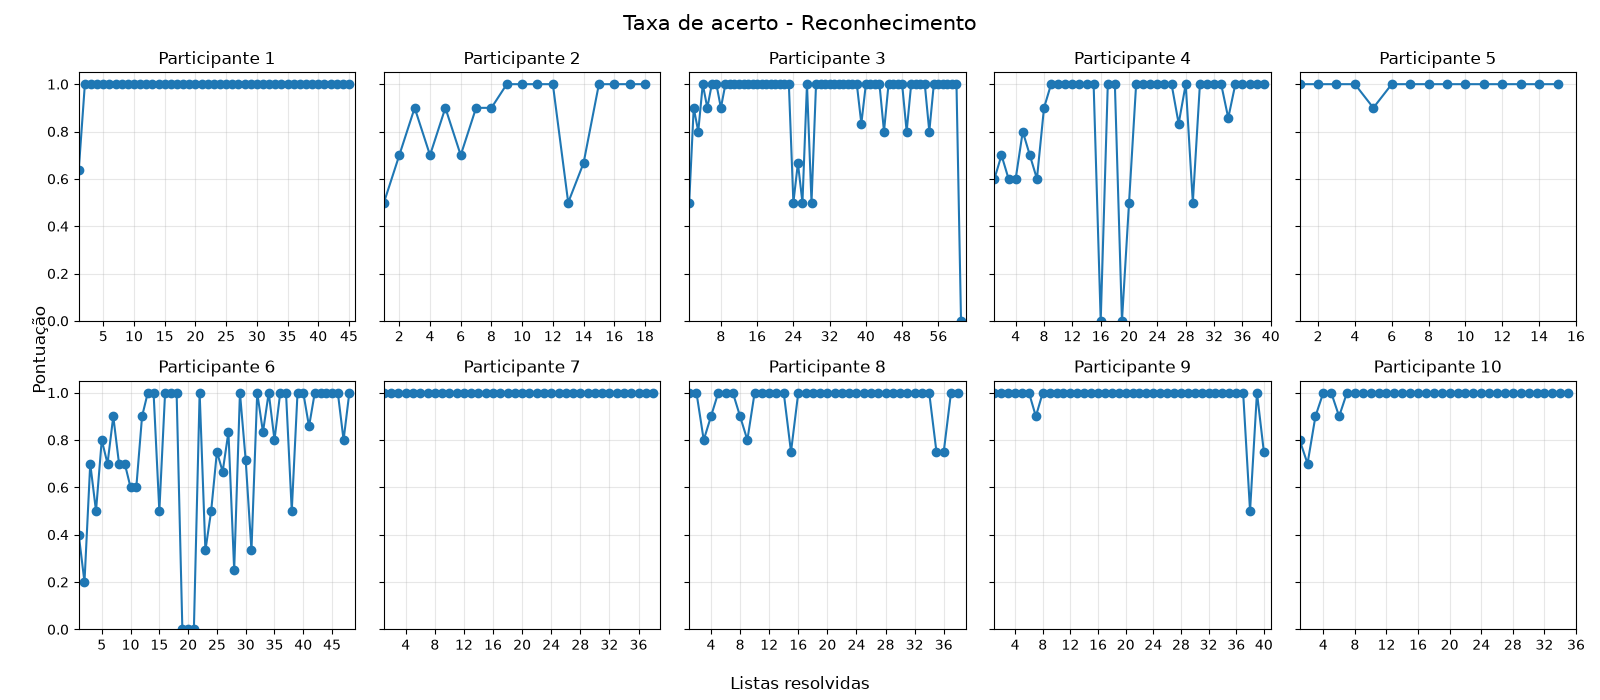
\includegraphics[width=0.9\textwidth]
    {images/appendix_A/desempenho_recon.png}
    \caption{Desempenho geral no módulo de Reconhecimento}
    \label{fig:desempenho_recon}
\end{figure}

\begin{figure}[H]
    \centering
    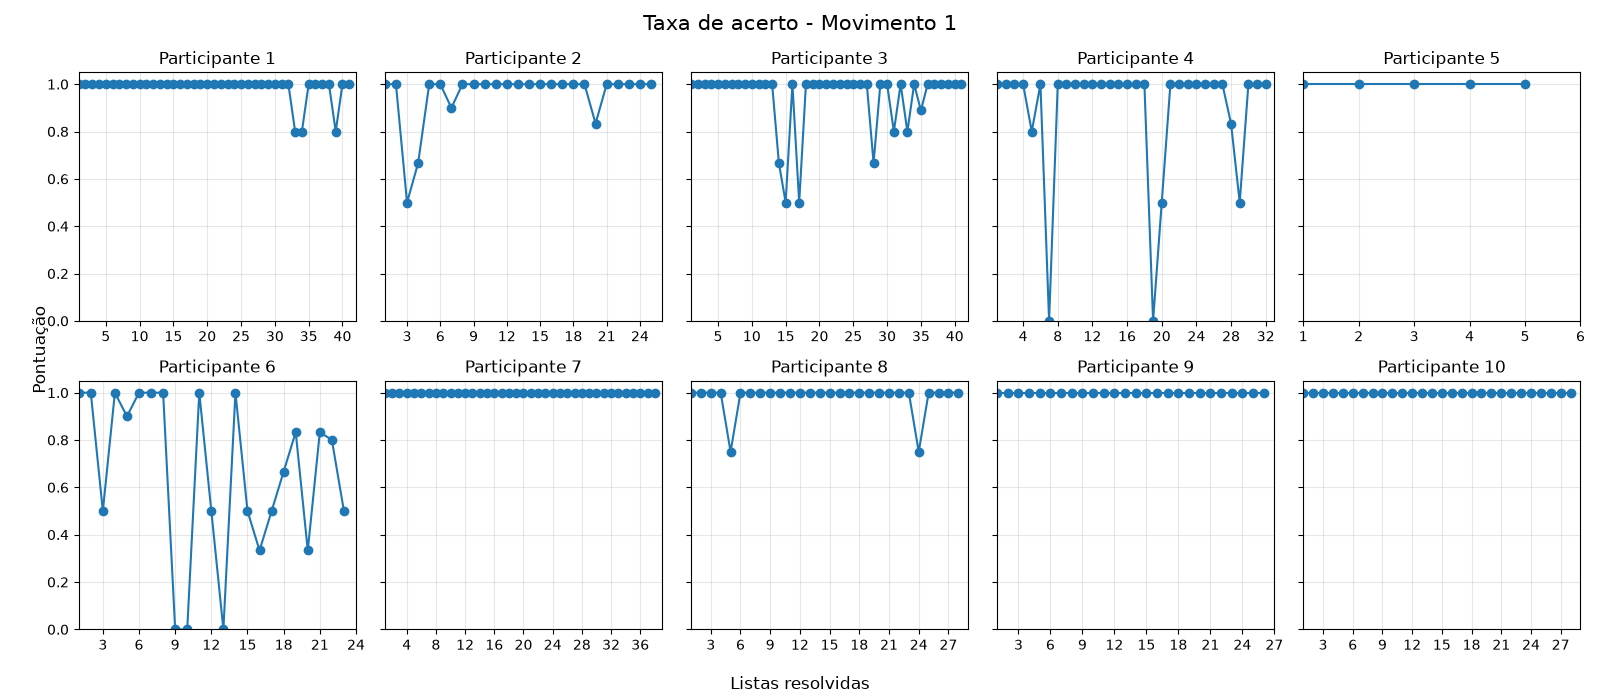
\includegraphics[width=0.9\textwidth]
    {images/appendix_A/desempenho_move1.png}
    \caption{Desempenho geral no módulo de Movimento 1}
    \label{fig:desempenho_move1}
\end{figure}

\begin{figure}[H]
    \centering
    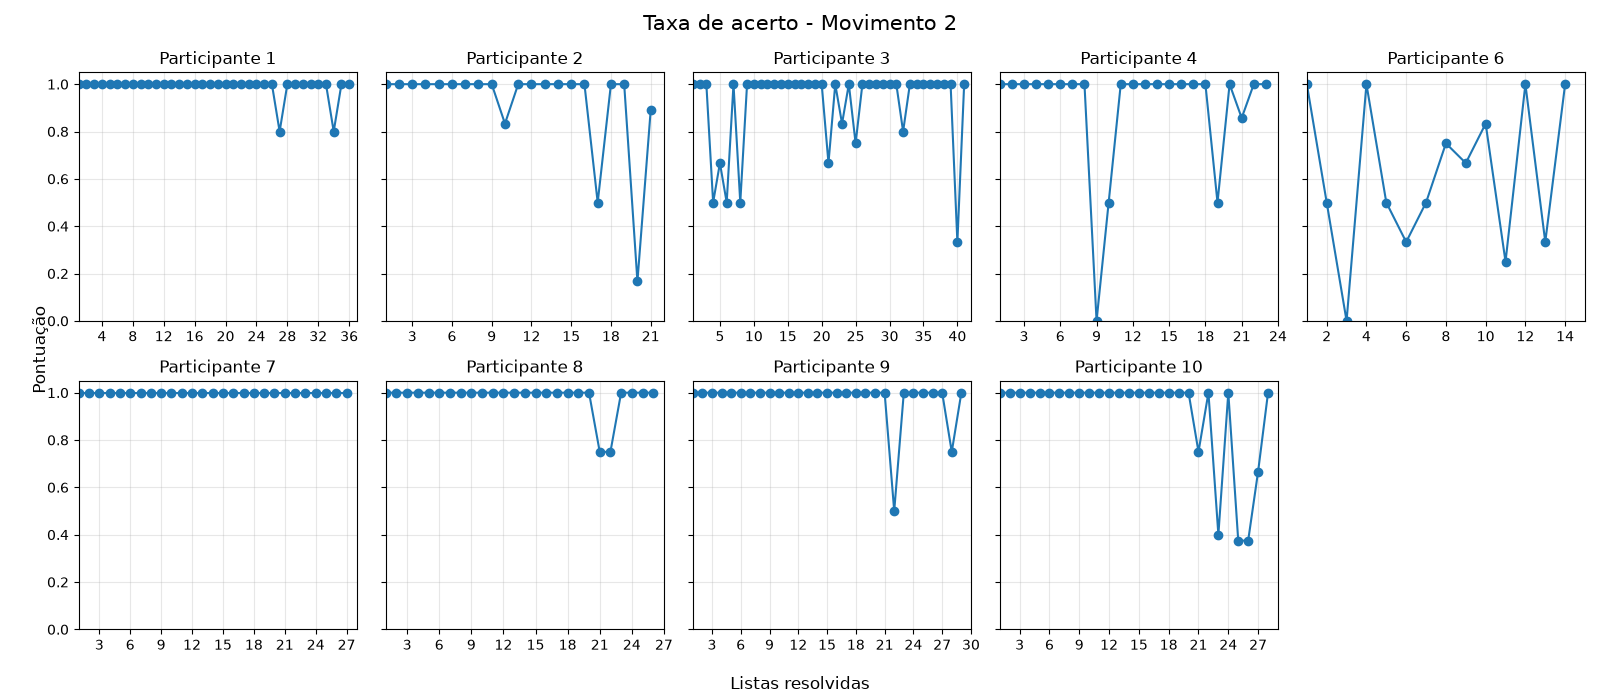
\includegraphics[width=0.9\textwidth]
    {images/appendix_A/desempenho_move2.png}
    \caption{Desempenho geral no módulo de Movimento 2}
    \label{fig:desempenho_move2}
\end{figure}

\begin{figure}[H]
    \centering
    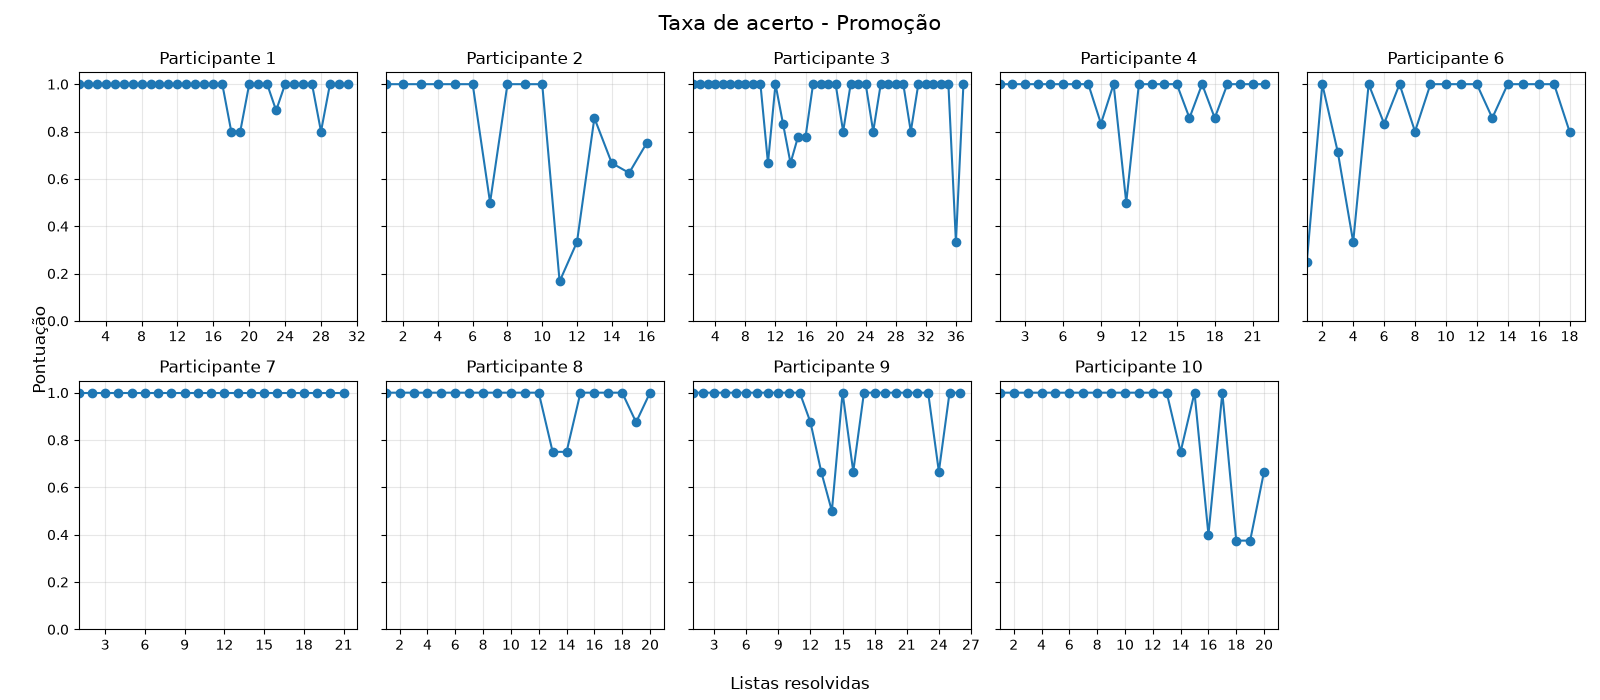
\includegraphics[width=0.9\textwidth]
    {images/appendix_A/desempenho_promo.png}
    \caption{Desempenho geral no módulo de Promoção}
    \label{fig:desempenho_promo}
\end{figure}

\begin{figure}[H]
    \centering
    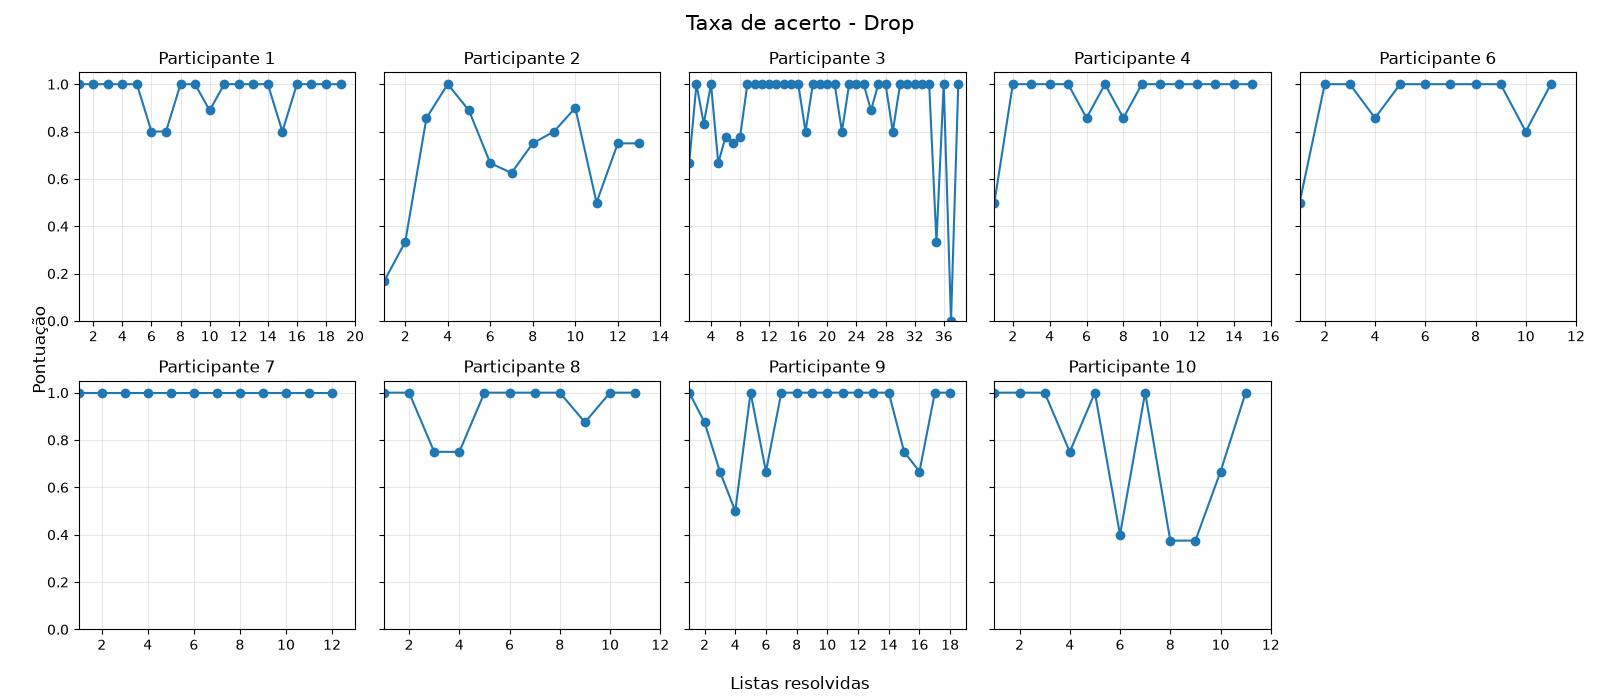
\includegraphics[width=0.9\textwidth]
    {images/appendix_A/desempenho_drop.png}
    \caption{Desempenho geral no módulo de Drop}
    \label{fig:desempenho_drop}
\end{figure}

\begin{figure}[H]
    \centering
    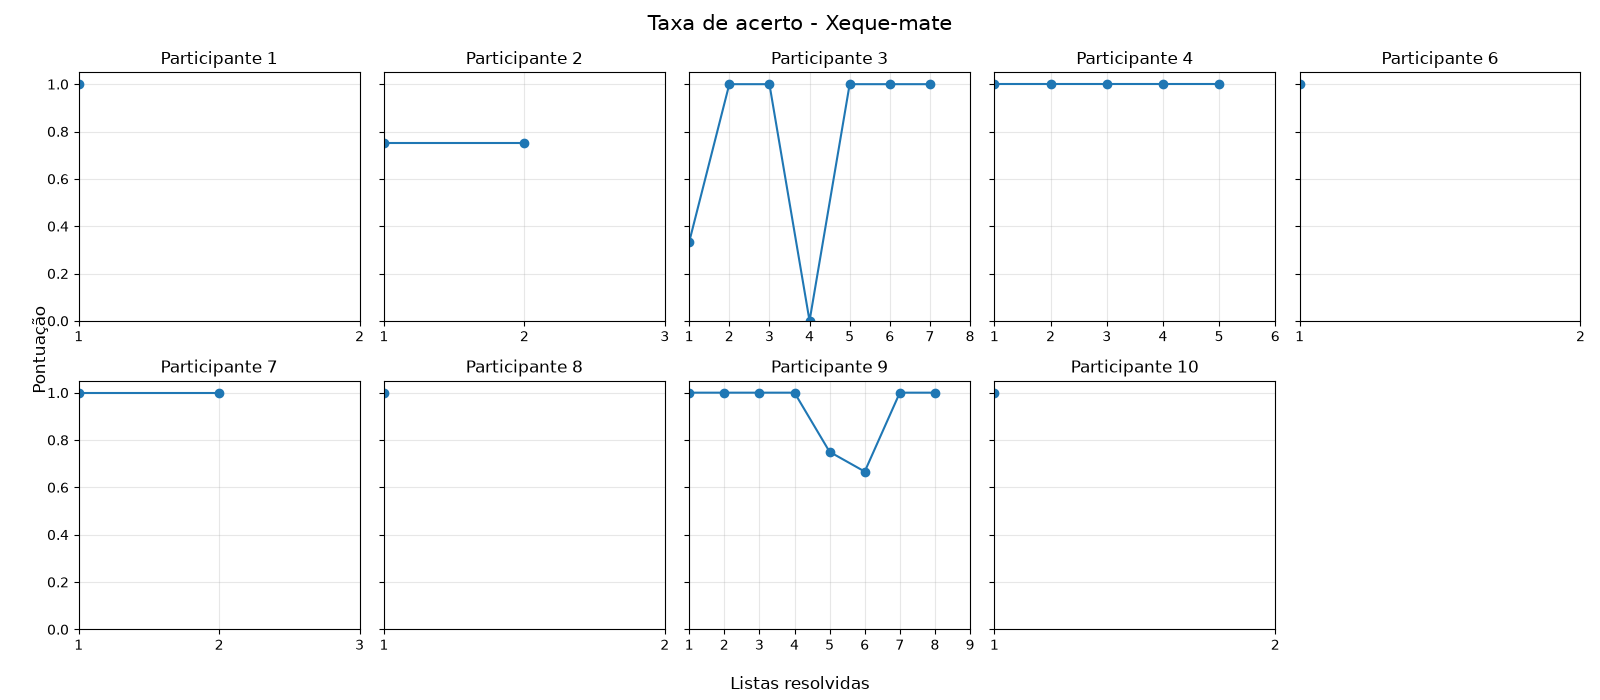
\includegraphics[width=0.9\textwidth]
    {images/appendix_A/desempenho_check.png}
    \caption{Desempenho geral no módulo de Xeque-mate}
    \label{fig:desempenho_check}
\end{figure}

\section{Tempo médio de resposta por módulo}
\label{ap:avg_response_time}
\begin{figure}[H]
    \centering
    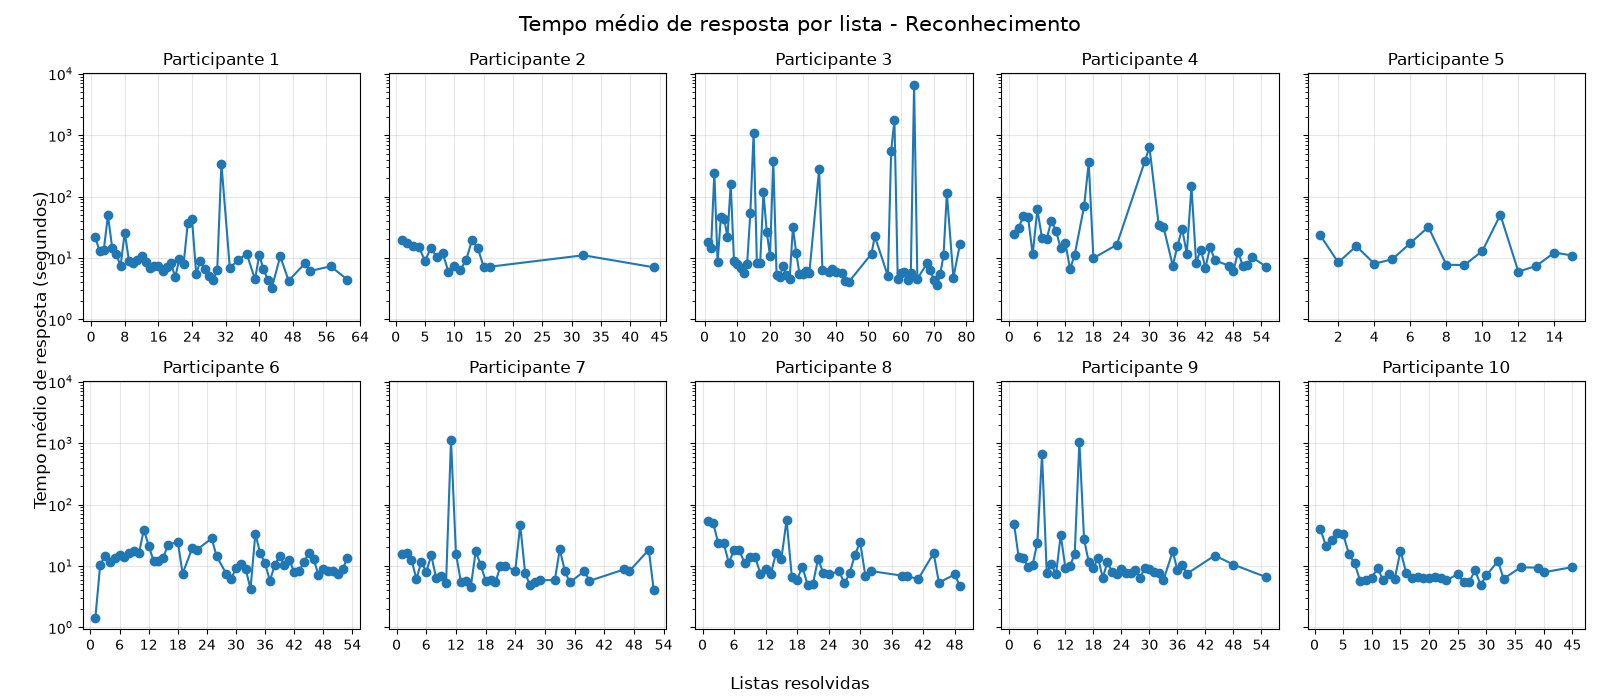
\includegraphics[width=0.9\textwidth]
    {images/appendix_A/response_time_recon.png}
    \caption{Tempo médio de resposta do módulo de Reconhecimento}
    \label{fig:response_time_recon}
\end{figure}

\begin{figure}[H]
    \centering
    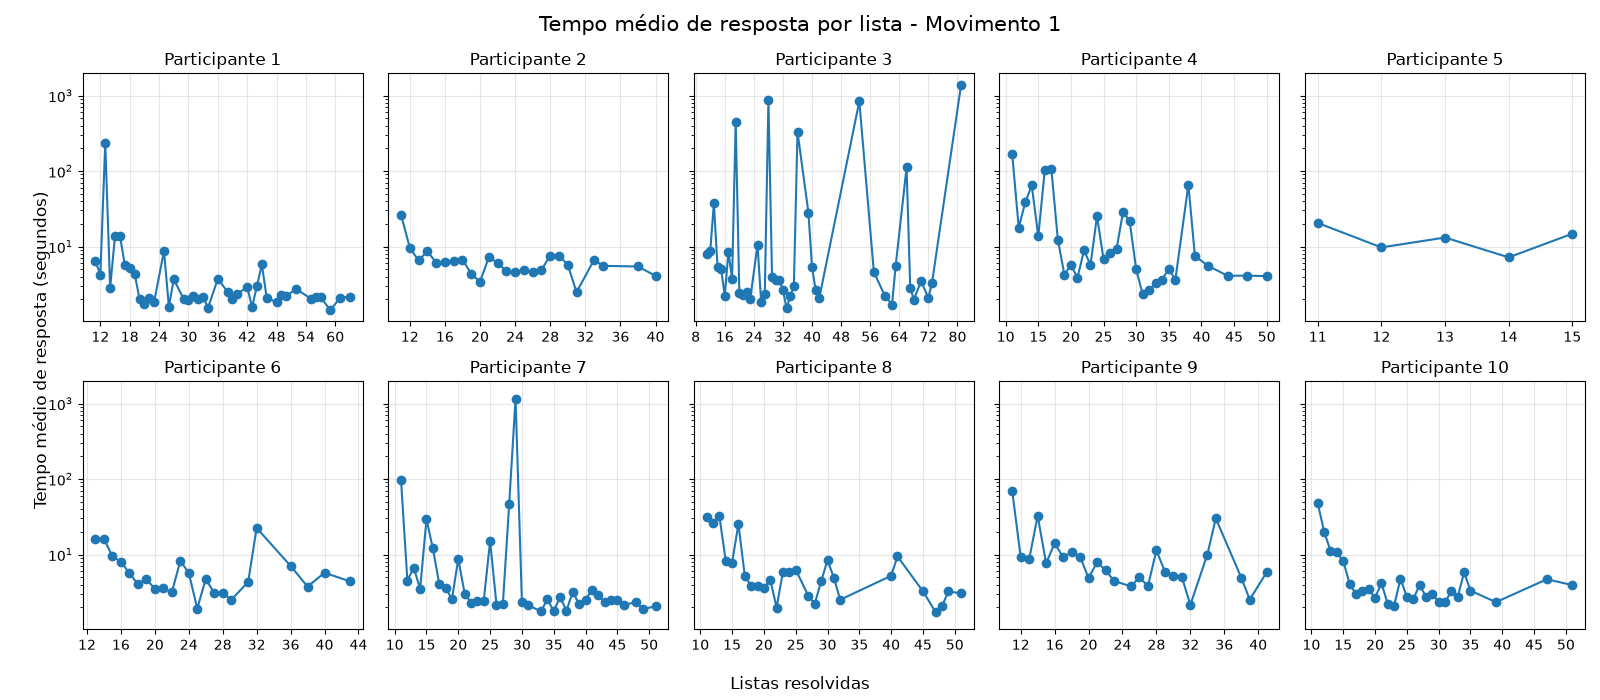
\includegraphics[width=0.9\textwidth]
    {images/appendix_A/response_time_move1.png}
    \caption{Tempo médio de resposta do módulo de Movimento 1}
    \label{fig:response_time_move1}
\end{figure}

\begin{figure}[H]
    \centering
    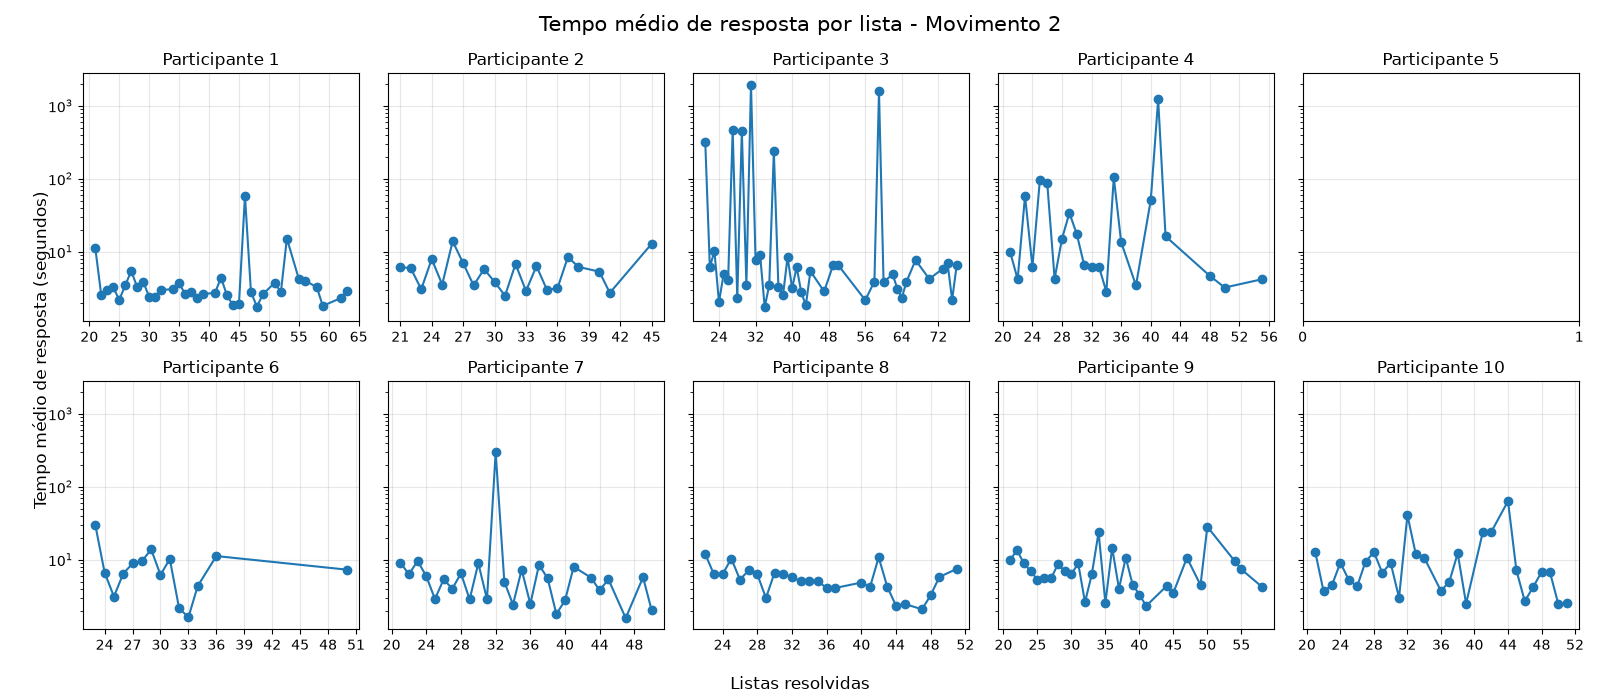
\includegraphics[width=0.9\textwidth]
    {images/appendix_A/response_time_move2.png}
    \caption{Tempo médio de resposta do módulo de Movimento 2}
    \label{fig:response_time_move2}
\end{figure}

\begin{figure}[H]
    \centering
    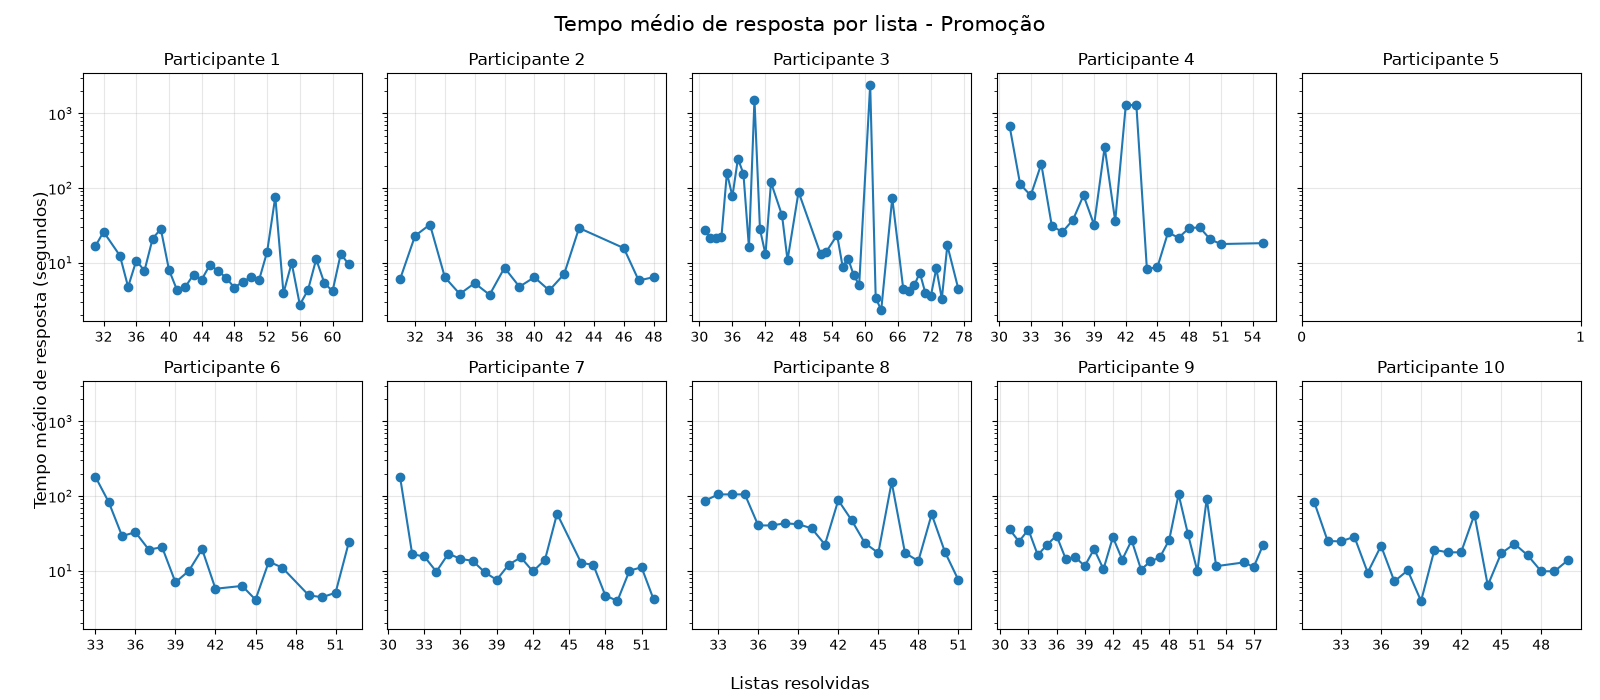
\includegraphics[width=0.9\textwidth]
    {images/appendix_A/response_time_promo.png}
    \caption{Tempo médio de resposta do módulo de Promoção}
    \label{fig:response_time_promo}
\end{figure}

\begin{figure}[H]
    \centering
    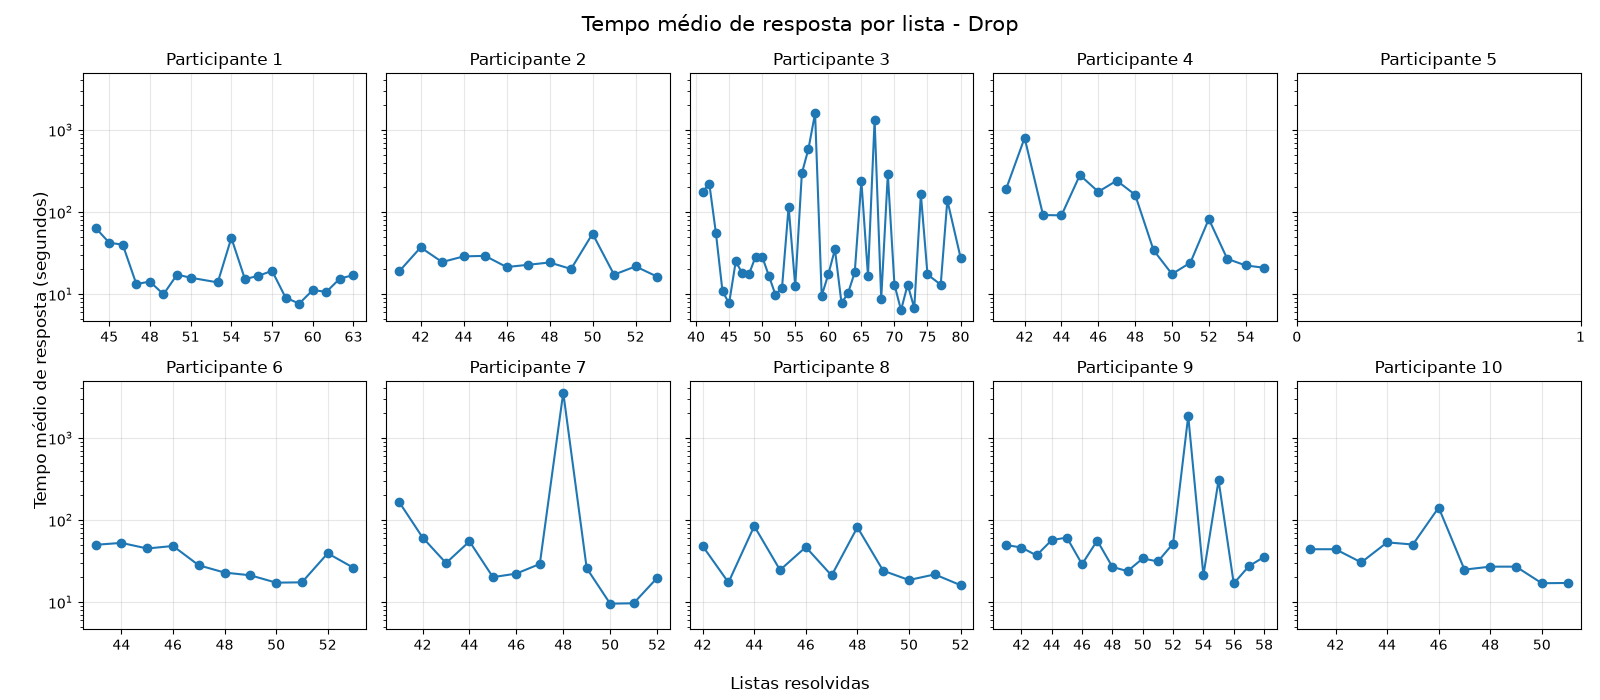
\includegraphics[width=0.9\textwidth]
    {images/appendix_A/response_time_drop.png}
    \caption{Tempo médio de resposta do módulo de Drop}
    \label{fig:response_time_drop}
\end{figure}

\begin{figure}[H]
    \centering
    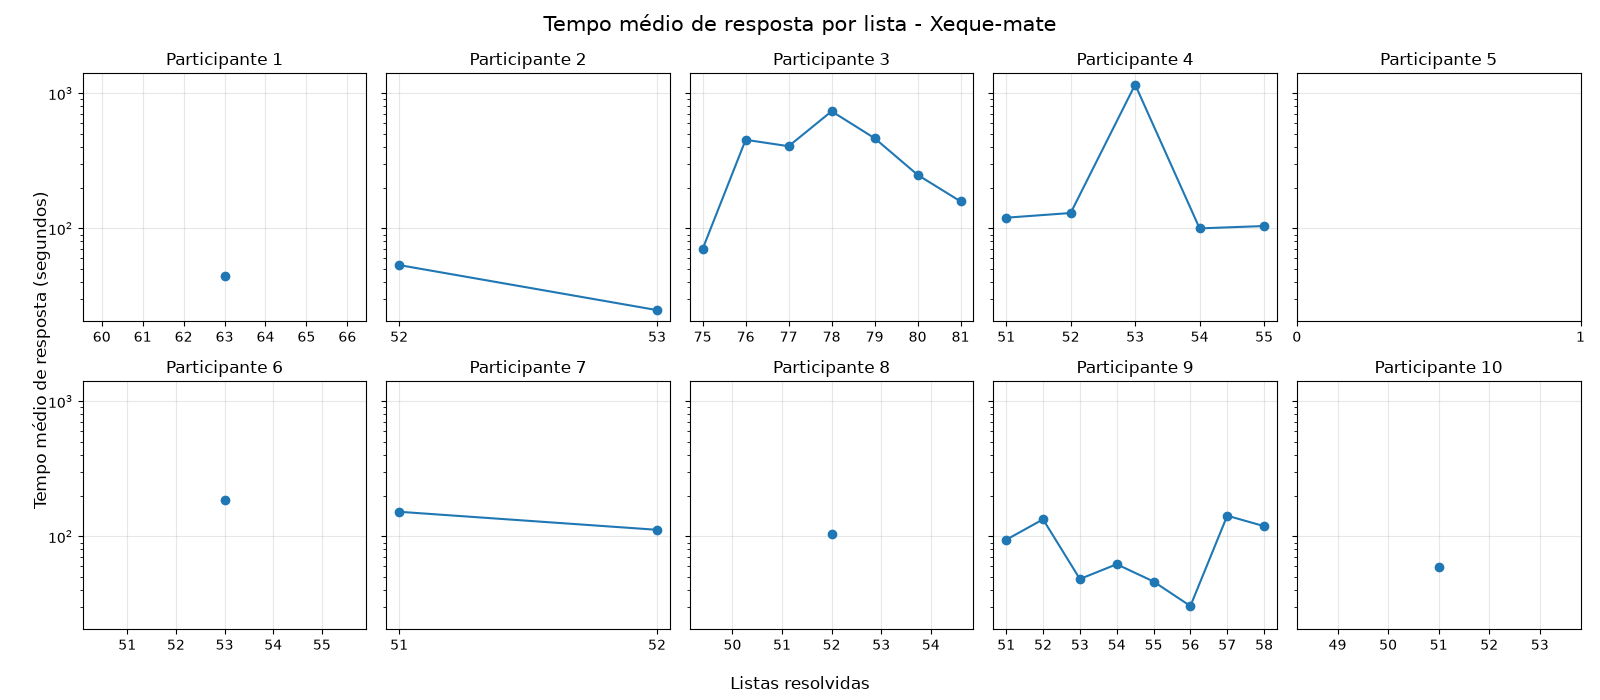
\includegraphics[width=0.9\textwidth]
    {images/appendix_A/response_time_check.png}
    \caption{Tempo médio de resposta do módulo de Xeque-mate}
    \label{fig:response_time_check}
\end{figure}

\section{Distribuição das probabilidades dos módulos}
\label{ap:modules_probs}

\begin{figure}[H]
    \centering
    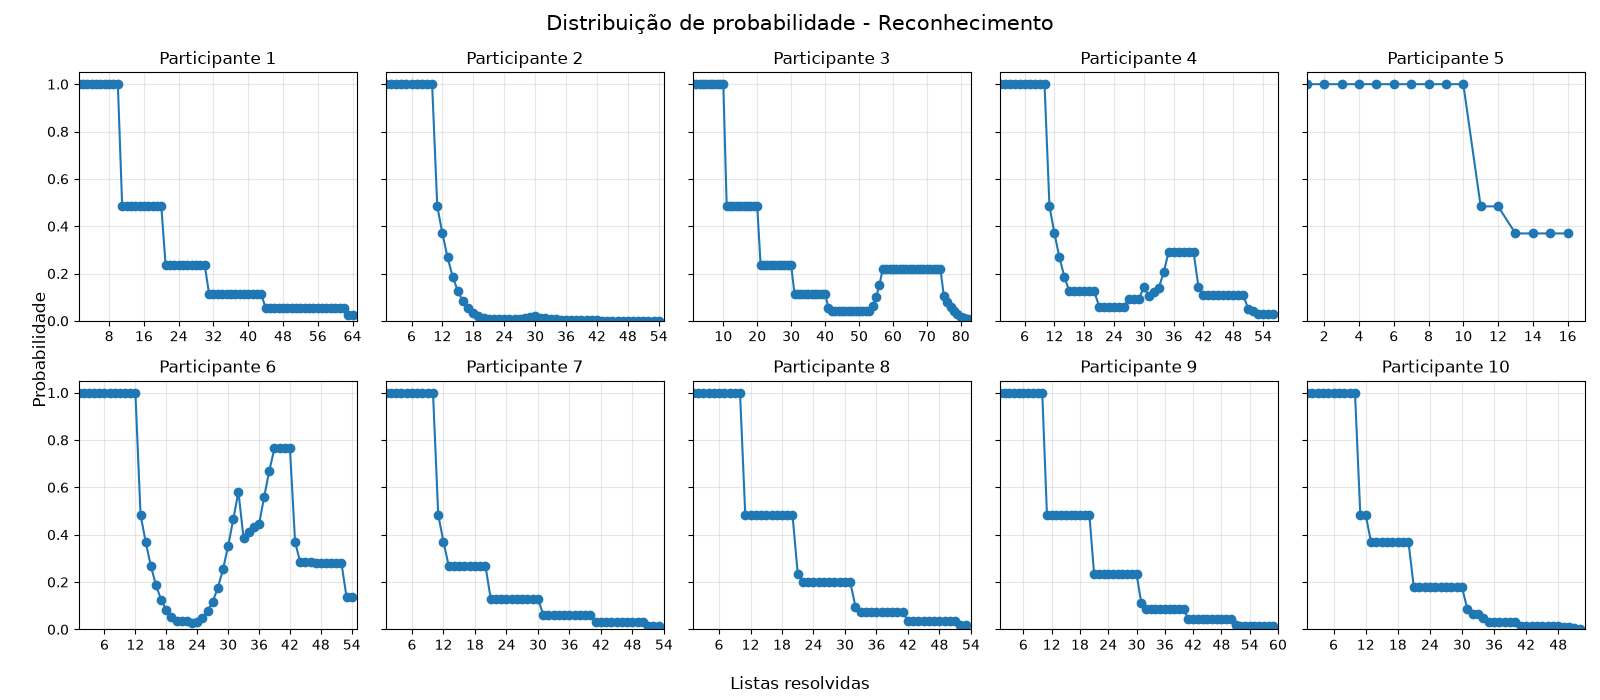
\includegraphics[width=0.9\textwidth]
    {images/appendix_A/probs_recon.png}
    \caption{Distribuição de probabilidades do módulo de Reconhecimento}
    \label{fig:probs_recon}
\end{figure}

\begin{figure}[H]
    \centering
    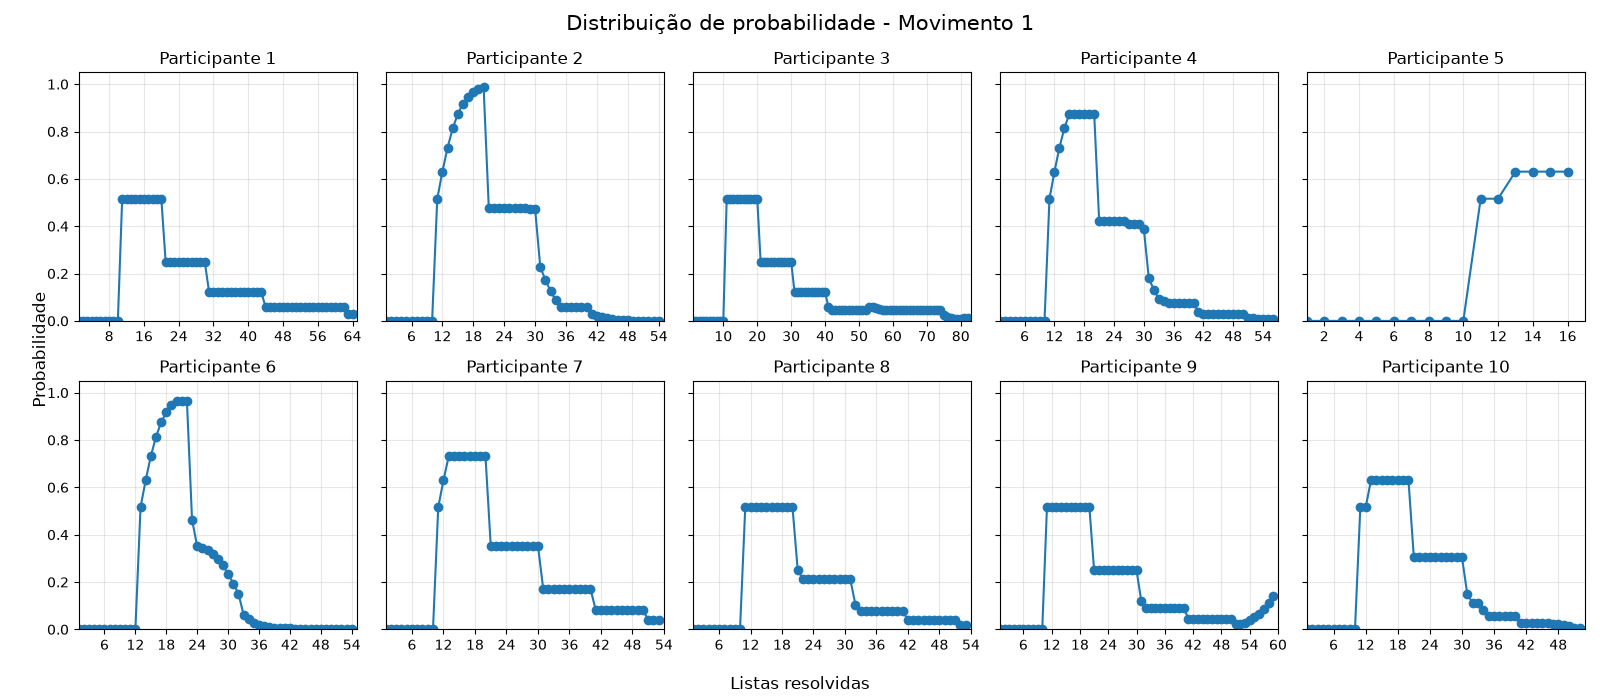
\includegraphics[width=0.9\textwidth]
    {images/appendix_A/probs_move1.png}
    \caption{Distribuição de probabilidades do módulo de Movimento 1}
    \label{fig:probs_move1}
\end{figure}

\begin{figure}[H]
    \centering
    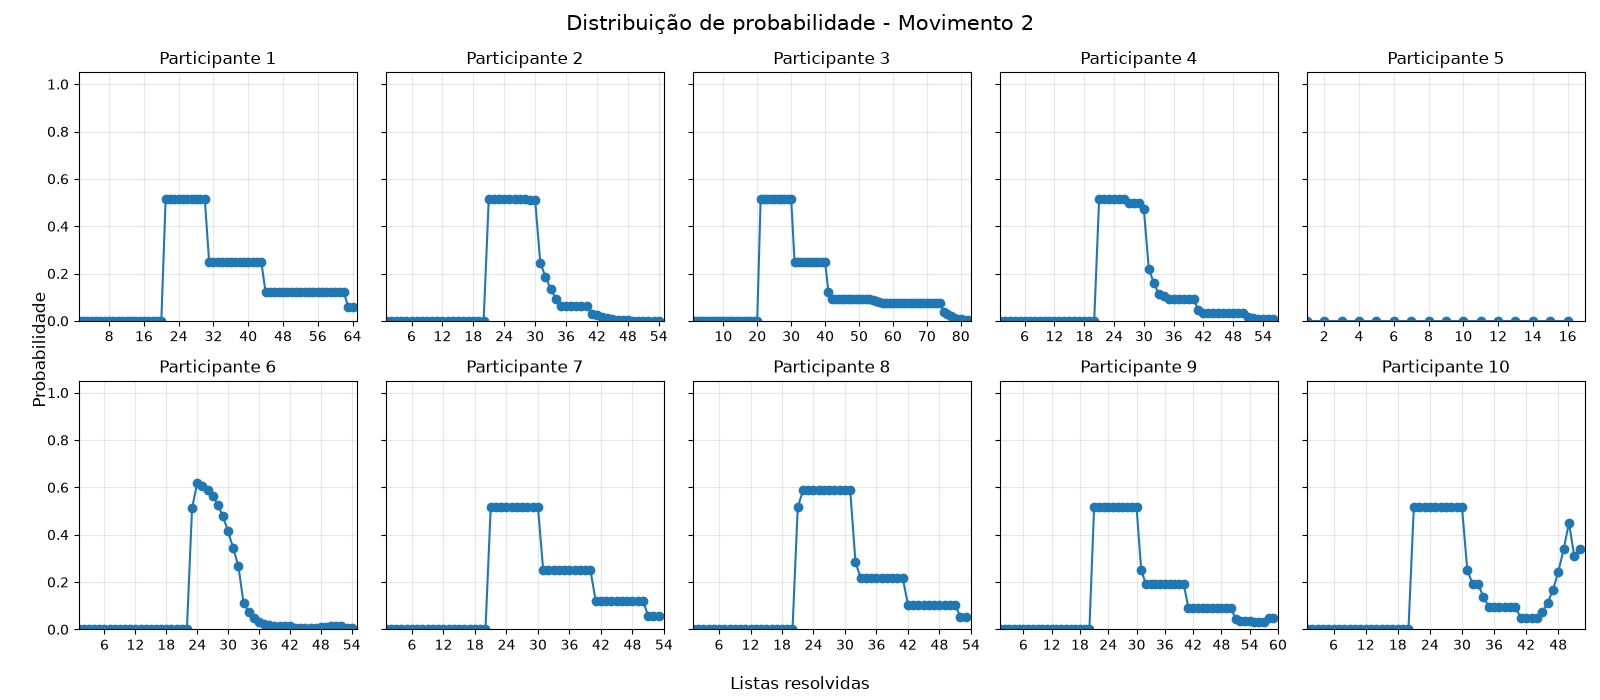
\includegraphics[width=0.9\textwidth]
    {images/appendix_A/probs_move2.png}
    \caption{Distribuição de probabilidades do módulo de Movimento 2}
    \label{fig:probs_move2}
\end{figure}

\begin{figure}[H]
    \centering
    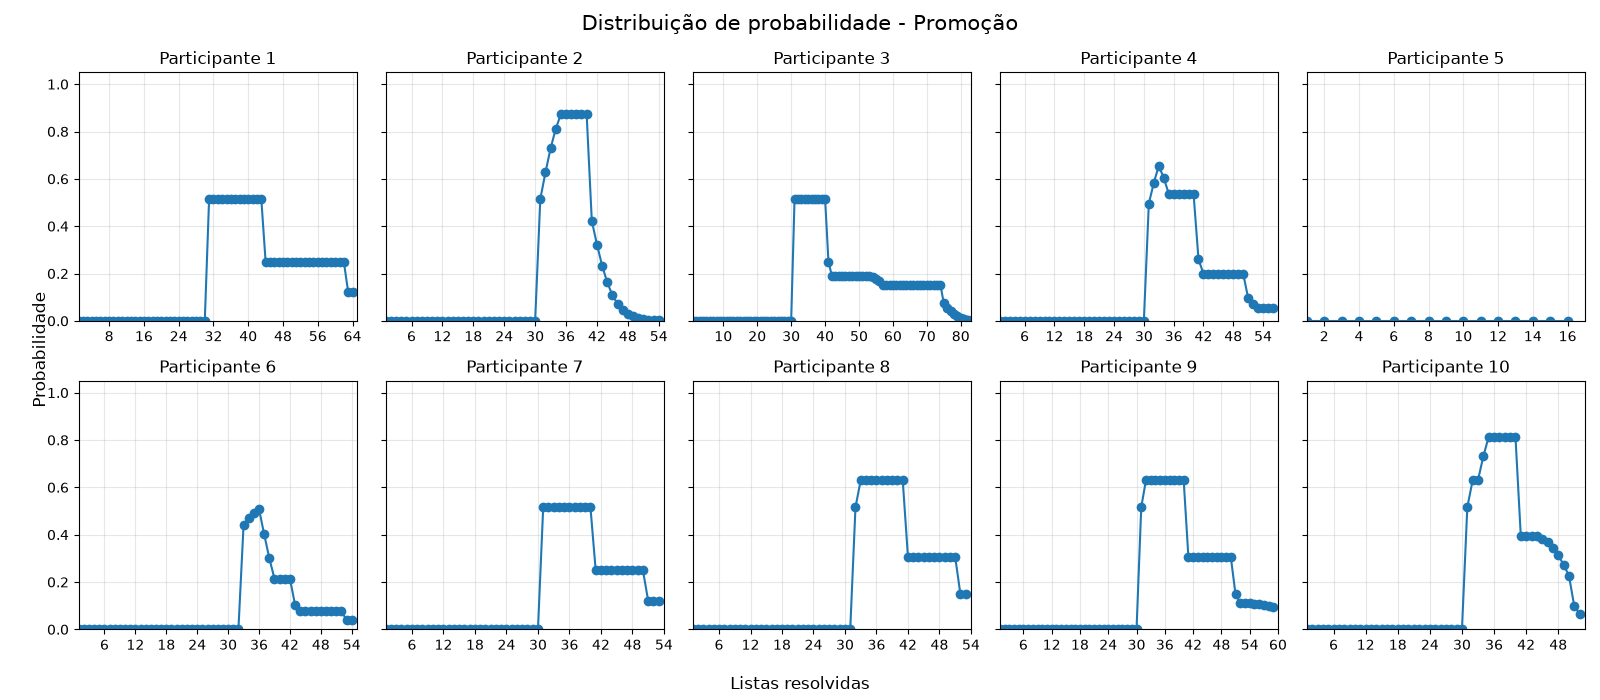
\includegraphics[width=0.9\textwidth]
    {images/appendix_A/probs_promo.png}
    \caption{Distribuição de probabilidades do módulo de Promoção}
    \label{fig:probs_promo}
\end{figure}

\begin{figure}[H]
    \centering
    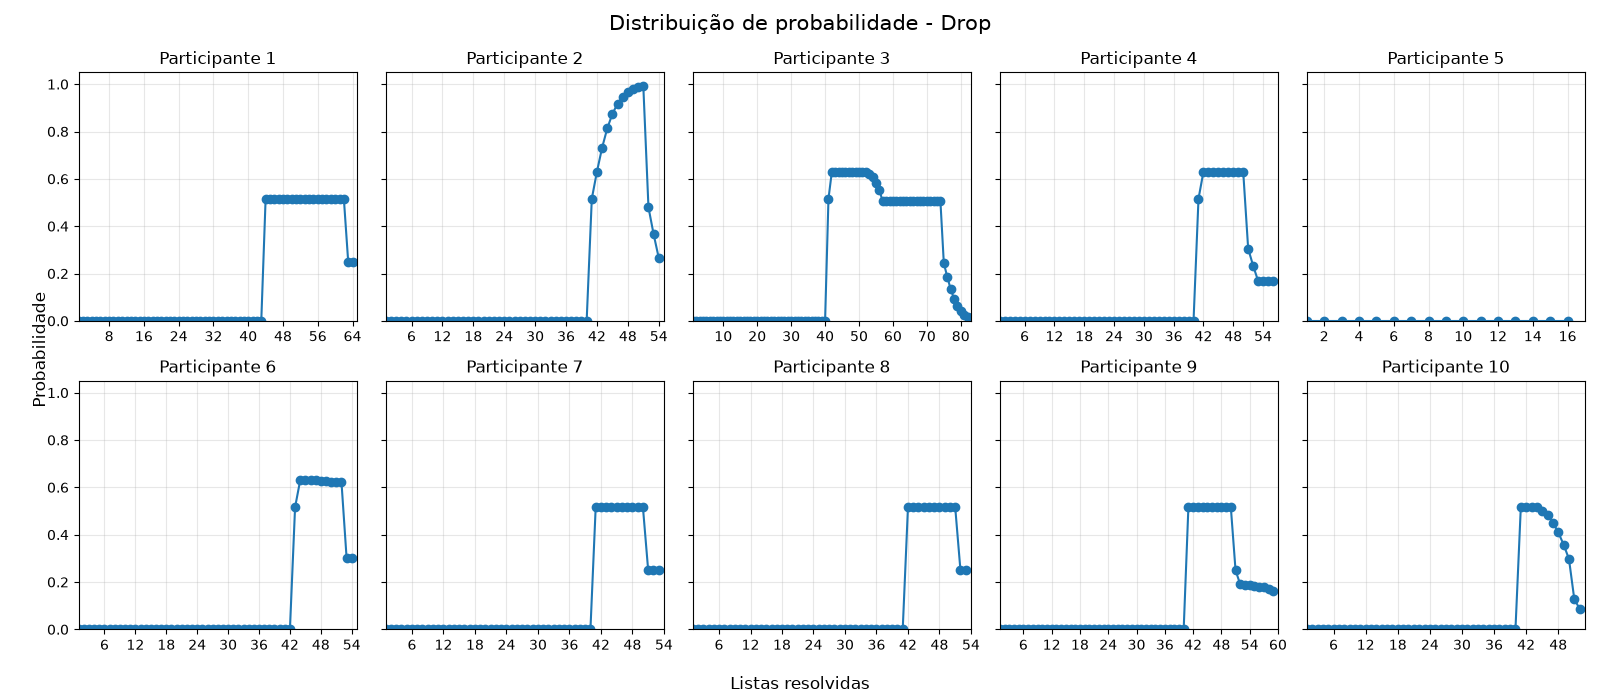
\includegraphics[width=0.9\textwidth]
    {images/appendix_A/probs_drop.png}
    \caption{Distribuição de probabilidades do módulo de Drop}
    \label{fig:probs_drop}
\end{figure}

\begin{figure}[H]
    \centering
    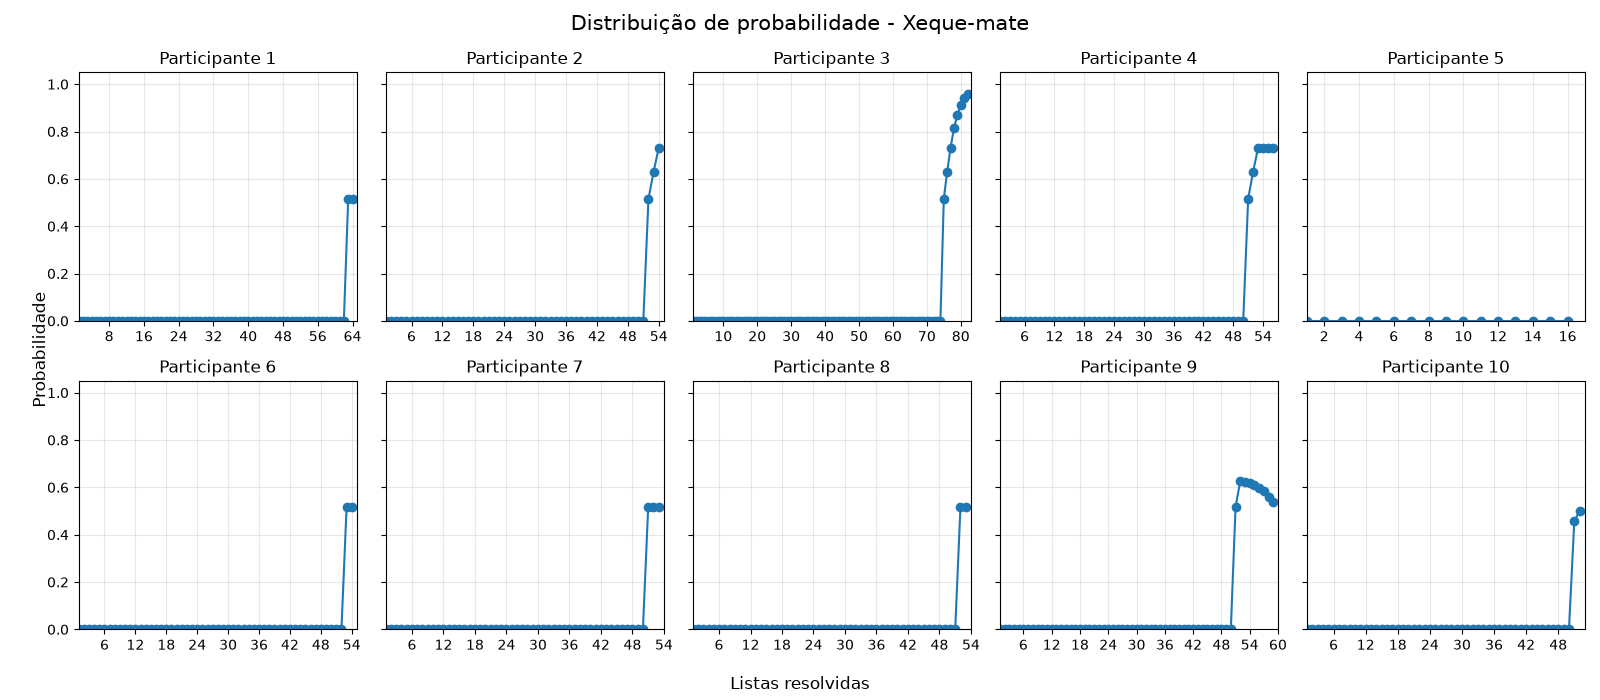
\includegraphics[width=0.9\textwidth]
    {images/appendix_A/probs_check.png}
    \caption{Distribuição de probabilidades do módulo de Xeque-mate}
    \label{fig:probs_check}
\end{figure}
\pagestyle{mainmatter}

%%%%%%%%%%%%%%% SEÇÕES FINAIS (BIBLIOGRAFIA E ÍNDICE REMISSIVO) %%%%%%%%%%%%%%%%
\backmatter

\pagestyle{backmatter}

% Espaço adicional no sumário antes das referências / índice remissivo
\addtocontents{toc}{\vspace{2\baselineskip plus .5\baselineskip minus .5\baselineskip}}

\printbibliography[
  title=\refname\label{sec:bib},
  heading=bibintoc,
]

\printindex

\end{document}